\documentclass[a4paper, 11pt, oneside]{thesis}  % Use the "Thesis" style, based on the ECS Thesis style by Steve Gunn
%
% Put your figures in this directory
\graphicspath{Figures/}  % Location of the graphics files (set up for graphics to be in PDF format)
%

% Include any extra LaTeX packages required
%\usepackage[square, numbers, comma, sort&compress]{natbib}  % Use the "Natbib" style for the references in the Bibliography
\usepackage[square, numbers, comma, sort&compress]{natbib}  % Use the "Natbib" style for the references in the Bibliography
\usepackage{verbatim}  % Needed for the "comment" environment to make LaTeX comments
\usepackage{vector}  % Allows "\bvec{}" and "\buvec{}" for "blackboard" style bold vectors in maths
\hypersetup{urlcolor=blue, colorlinks=true}  % Colours hyperlinks in blue, but this can be distracting if there are many links.

\usepackage[table]{xcolor}

\usepackage[toc,title]{appendix}
\usepackage{paralist}

\usepackage{mathtools}
\usepackage{amsmath,amssymb,amsfonts}
\usepackage{algorithm}
\usepackage{algorithmic}
\usepackage{color}
% nicer urls that break at the end of the page
\usepackage{url}
\usepackage{graphicx}
\usepackage{adjustbox}
\usepackage{enumerate}
\usepackage{subcaption}
\usepackage{pgfgantt}
\usepackage[final]{pdfpages}

\usepackage{graphicx}
\usepackage{placeins}
\usepackage{stmaryrd}

\usepackage{hyperref}
\hypersetup{
    colorlinks=true,
    linkcolor=blue,
    filecolor=magenta,      
    urlcolor=blue,
}

% definitions
% some common definitions:
%==============================================================================

% environments
%==============================================================================
%\newtheorem{theorem}{Theorem}
%\newtheorem{proposition}{Proposition}
%\newtheorem{lemma}{Lemma}
%\newtheorem{corollary}{Corollary}
%%\newtheorem{definition}{Definition}
%\newtheorem{remark}{Remark}
%\newtheorem{example}{Example}
%\newtheorem{summary}{Summary}
%\newtheorem*{summary*}{Summary}
%
%\declaretheoremstyle[
%headpunct={},
%headfont=\bfseries,%\itshape,
%notefont=\bfseries,%\itshape,notebraces={}{},
%bodyfont=\normalfont,
%%headformat=\underline{\NAME~\NUMBER:\NOTE}
%headformat=\NAME~\NUMBER:\NOTE.
%]{def}
%\declaretheorem[style=def]{definition}
%
%\def\sectionautorefname{Section}

\renewcommand{\chapterautorefname}{Chapter}
\renewcommand{\sectionautorefname}{Section}
\renewcommand{\subsectionautorefname}{Section}

% commands
%==============================================================================
\newcommand{\fml}[1]{{\mathcal{#1}}}
\newcommand{\mfrk}[1]{{\mathfrak{#1}}}
\newcommand{\set}[1]{\{ #1 \}}
\newcommand{\fcall}[1]{{\texttt{#1}}}
\newcommand{\vect}[1]{\mathbf{#1}}
\newcommand{\tn}[1]{\textnormal{#1}}
\newcommand{\mbf}[1]{\ensuremath\mathbf{#1}}
\newcommand{\mbb}[1]{\ensuremath\mathbb{#1}}
\newcommand{\msf}[1]{\ensuremath\mathsf{#1}}
\newcommand{\mnm}[1]{\ensuremath\mathnormal{#1}}
\newcommand{\vdef}{\ensuremath\mathsf{var}}
\newcommand{\suffix}{\ensuremath\mathsf{suffix}}
\newcommand{\tbf}[1]{\textbf{#1}}
\newcommand{\tsf}[1]{\textsf{#1}}
\newcommand{\tl}[1]{{\small\textsl{#1}}}
\newcommand{\lit}[1]{{\small\ensuremath\tn{#1}\xspace}}
\newcommand{\nlit}[1]{{\small\ensuremath\neg\tn{#1}\xspace}}
\newcommand{\eqlit}[2]{{\small(\ensuremath\tn{#1}=\tn{#2})\xspace}}
\newcommand{\noarg}{\phantom{~}}
\newcommand{\hlit}[1]{\ensuremath\textcolor{tblue2}{\tn{\bfseries{#1}}}\xspace}
\newcommand{\nhlit}[1]{\ensuremath\textcolor{tblue2}{\bm{\neg}\tn{\bfseries{#1}}}\xspace}
%\newcommand{\model}[1]{\mathfrak{#1}}
\newcommand{\ignore}[1]{}

\newcommand{\ffa}{\textrm{ffa}}
\newcommand{\ffalabel}[1]{\textrm{FFA}$_{\textrm{#1}}$}
\newcommand{\wffalabel}[1]{\textrm{WFFA}$_{\textrm{#1}}$}
\newcommand{\fcfa}{\textrm{fcfa}}
\newcommand{\wffa}{\textrm{wffa}}
\newcommand{\axps}{\ensuremath\mbb{A}}
\newcommand{\cxps}{\ensuremath\mbb{C}}

\DeclareMathOperator*{\entails}{\vDash}
\DeclareMathOperator*{\nentails}{\nvDash}
\DeclareMathOperator*{\lequiv}{\leftrightarrow}
\DeclareMathOperator*{\limply}{\rightarrow}

\newcommand{\ddp}{\tn{D}^{\tn{P}}}
%
\newcommand{\ttwop}{\Theta_2^\tn{P}}
\newcommand{\dtwop}{\Delta_2^\tn{P}}
\newcommand{\stwop}{\Sigma_2^\tn{P}}
%
\newcommand{\tthreep}{\Theta_3^\tn{P}}
\newcommand{\dthreep}{\Delta_3^\tn{P}}
\newcommand{\sthreep}{\Sigma_3^\tn{P}}
\newcommand{\papsd}{$P=(\fml{V},\fml{H},\fml{E},\fml{F})$\xspace}
\newcommand{\papdef}{$P=(\fml{V},\fml{H},\fml{E},\fml{F},c)$\xspace}
\newcommand{\papdefn}[1]{$P_{#1}=(\fml{V},\fml{H},\fml{E},\fml{F},c)$\xspace}

\newcommand{\cond}{d} % condition value
\newcommand{\sep}{s}  % separator lists

\newcommand{\ac}[1]{\left[\!\left[ #1 \right]\!\right]}

% qed
%==============================================================================
\def\squareforqed{\hbox{\rlap{$\sqcap$}$\sqcup$}}
\def\qed{\ifmmode\squareforqed\else{\unskip\nobreak\hfil
\penalty50\hskip1em\null\nobreak\hfil\squareforqed
\parfillskip=0pt\finalhyphendemerits=0\endgraf}\fi}

\newcommand{\anote}[1]{$\llbracket$\textcolor{tred3}{alexey}:~~{\sl\textcolor{tdgray1}{#1}}$\rrbracket$}
\newcommand{\pnote}[1]{$\llbracket$\textcolor{tred3}{peter}:~~{\sl\textcolor{tdgray1}{#1}}$\rrbracket$}
\newcommand{\jynote}[1]{$\llbracket$\textcolor{tred3}{jinqiang}:~~{\sl\textcolor{tdgray1}{#1}}$\rrbracket$}
\newcommand{\nocxp}[1]{#1}
\newcommand{\pjs}[1]{\pnote{#1}}

\newcommand*\boxmodpalettela[2]{\mathbin{\raisebox{0.1\height}{\scalebox{0.8}{{\fboxsep1pt\fbox{$#1\Leftarrow$}}}}}}
\newcommand*\boxla{\mathpalette\boxmodpalettela{}}
\newcommand*\boxmodpalettera[2]{\mathbin{\raisebox{0.1\height}{\scalebox{0.8}{{\fboxsep1pt\fbox{$#1\Rightarrow$}}}}}}
\newcommand*\boxra{\mathpalette\boxmodpalettera{}}
\newcommand{\frmeq}[1]{\begin{empheq}[box={\fboxsep=1.5pt\doublebox}]{flalign*}#1\end{empheq}}


\DeclareMathOperator*{\argmin}{arg\,min}
\DeclareMathOperator*{\argmax}{arg\,max}


\newcommand{\model}{\fml{M}}
\newcommand{\cfunc}{\kappa}
\newcommand{\feats}{\fml{F}}
\newcommand{\cfeats}{\mathbb{F}}
\newcommand{\clss}{\fml{K}}
\newcommand{\domain}{\mbb{D}}
\newcommand{\trees}{\mathfrak{T}}
\newcommand{\tree}{t}
\newcommand{\tnodes}{V}
\newcommand{\edges}{E}
\newcommand{\tnode}{\mathfrak{n}}
\newcommand{\tpath}{\fml{P}}
\newcommand{\apoints}{\fml{H}}
\newcommand{\axp}{\fml{X}}
\newcommand{\cxp}{\fml{Y}}
\newcommand{\mhs}{\textrm{MHS}}
\newcommand{\mins}{\textrm{mins}}
\newcommand{\hs}{\textrm{HS}}
\newcommand{\cnf}{\Phi}
\newcommand{\softcl}{\fml{S}}
\newcommand{\hardcl}{\fml{H}}
\newcommand{\thesistopic}{Explainable AI with the Use of Formal Reasoning}

%\newcommand{\newm}[1]{\textcolor{blue}{#1}}
\newcommand{\newm}[1]{#1}
\newcommand{\newmm}[1]{\textcolor{blue}{#1}}

% tango colors
%
% yellow
\definecolor{tyellow1}{HTML}{FCE94F}
\definecolor{tyellow2}{HTML}{EDD400}
\definecolor{tyellow3}{HTML}{C4A000}
%
% orange
\definecolor{torange1}{HTML}{FCAF3E}
\definecolor{torange2}{HTML}{F57900}
\definecolor{torange3}{HTML}{C35C00}
%
% brown
\definecolor{tbrown1}{HTML}{E9B96E}
\definecolor{tbrown2}{HTML}{C17D11}
\definecolor{tbrown3}{HTML}{8F5902}
%
% green
\definecolor{tgreen1}{HTML}{8AE234}
\definecolor{tgreen2}{HTML}{73D216}
\definecolor{tgreen3}{HTML}{4E9A06}
%
% blue
\definecolor{tblue1}{HTML}{729FCF}
\definecolor{tblue2}{HTML}{3465A4}
\definecolor{tblue3}{HTML}{204A87}
%
% purple
\definecolor{tpurple1}{HTML}{AD7FA8}
\definecolor{tpurple2}{HTML}{75507B}
\definecolor{tpurple3}{HTML}{5C3566}
%
% red
\definecolor{tred1}{HTML}{EF2929}
\definecolor{tred2}{HTML}{CC0000}
\definecolor{tred3}{HTML}{A40000}
%
% light gray
\definecolor{tlgray1}{HTML}{EEEEEC}
\definecolor{tlgray2}{HTML}{D3D7CF}
\definecolor{tlgray3}{HTML}{BABDB6}
%
% dark gray
\definecolor{tdgray1}{HTML}{888A85}
\definecolor{tdgray2}{HTML}{555753}
\definecolor{tdgray3}{HTML}{2E3436}



\newcommand\BlackCell[2]{%
    \multicolumn{1}{|m{#1}|}{\cellcolor{black}\textcolor{white}{#2}}
}
\newcommand\WhiteCell[2]{%
    \multicolumn{1}{|m{#1}|}{\cellcolor{white}\textcolor{black}{#2}}
}

%% ----------------------------------------------------------------
\begin{document}
\frontmatter      % Begin Roman style (i, ii, iii, iv...) page numbering

%
\UNIVERSITY{{Monash University}}
%
%%%%%%%%%%%%%%%%%%%%%%%%%%%%%%%%%%%%%%%%%%%%%%%%%%%%%%%%%%%%%%%%%%%%%%%%%
% Update your department and school here:
\school{{Faculty of Information Technology}}
\gradtime{{2024}}
%%%%%%%%%%%%%%%%%%%%%%%%%%%%%%%%%%%%%%%%%%%%%%%%%%%%%%%%%%%%%%%%%%%%%%%%%

%
%%%%%%%%%%%%%%%%%%%%%%%%%%%%%%%%%%%%%%%%%%%%%%%%%%%%%%%%%%%%%%%%%%%%%%%%%
% Set up the Title Page
% Change your thesis title and your information here
\title  {\thesistopic}
\authors  {Jinqiang Yu%\texorpdfstring
            %{\href{your web site or email address}{Author Name }}
            %{Author Name}
            }
\addresses  {\groupname\\\deptname\\\univname}  % Do not change this here, instead these must be set in the "Thesis.cls" file, please look through it instead
\date       {\today}
\subject    {}
\keywords   {Biometrics}
%%%%%%%%%%%%%%%%%%%%%%%%%%%%%%%%%%%%%%%%%%%%%%%%%%%%%%%%%%%%%%%%%%%%%%%%%

\maketitle
%% ----------------------------------------------------------------

\setstretch{1.3}  % It is better to have smaller font and larger line spacing than the other way round

% Define the page headers using the FancyHdr package and set up for one-sided printing
\fancyhead{}  % Clears all page headers and footers
\rhead{\thepage}  % Sets the right side header to show the page number
\lhead{}  % Clears the left side page header

\pagestyle{fancy}  % Finally, use the "fancy" page style to implement the FancyHdr headers

\clearpage
%\newm{
\color{blue}
\textbf{Changes}

\begin{itemize}
	\item Abstract:
		\begin{itemize}
			\item Changed ``advancements'' to ``advances''
			\item Added a sentence introducing what intrinsic and post-hoc methods are.
			\item Minor fix
		\end{itemize}
	\item \autoref{sec:achiml}:
		\begin{itemize}
			\item Paraphrased the last paragraph.
			\item Add a sentence to mention existing governmental regulations and
				recommendations on AI.
				\item Minor fix.
		\end{itemize}
	\item \autoref{sec:risexai}:
		\begin{itemize}
			\item Clarified which references are surveys and which ones are papers.
		\end{itemize}
	\item \autoref{sec:motiv}:
		\begin{itemize}
			\item Mentioned Formal XAI~(FXAI) is an model-specific approach. (FXAI
				$\neq$ model-specific approach because some heuristic approaches are
				also model specific, such as TreeSHAP.)
			\item Added more context in contribution 3
			\item Minor fix.
		\end{itemize}
	\item \autoref{sec:rq}:
		\begin{itemize}
			\item Adjusted section counters.
			\item Updated publications
			\item Added a sentence in contribution 1 to describe our approach.
			\item Minor fix.
		\end{itemize}
	\item Section ``Publications during enrolment''
		\begin{itemize}
			\item Text and attached paper: Replaced the arxiv version of our paper ``Anytime Approximate Formal
				Feature Attribution.'' by the SAT conference paper.
			\item Text and attached paper: Replaced the Just-in-time explainer paper
				with the latest version. 
		\end{itemize}
	\item Removed text related to examiners Section ``Acknowledgement''.
	
\end{itemize}
%}
\color{black}

\clearpage

%% ----------------------------------------------------------------
% The copyright Page
% https://www.monash.edu/graduate-research/examination/publication
% https://www.monash.edu/rlo/graduate-research-writing/write-the-thesis
% https://www.monash.edu/rlo/graduate-research-writing/write-the-thesis/writing-the-thesis-chapters/structuring-a-long-text
%\copyrightnotice{

% \addtocontents{toc}{\vspace{1em}}  % Add a gap in the Contents, for aesthetics

\section*{Copyright notice}
\addtotoc{Copyright notice}

%Insert one of the following notices.
%
%Notice 1
%
%\textsuperscript{\textcopyright  \authornames (2024).}
%
%The second notice certifies the appropriate use of any third-party material in the thesis. Students choosing to deposit their thesis into the restricted access section of the repository are not required to complete Notice 2. 
%
%Notice 2

%\textsuperscript{\textcopyright  \authornames (2024).}
\text{\textcopyright  \authornames (2024).}

I certify that I have made all reasonable efforts to secure copyright permissions for third-party content included in this thesis and have not knowingly added copyright content to my work without the owner's permission.


%}

\clearpage  % copyright ended, start a new page
% https://www.monash.edu/graduate-research/examination/publication
% https://www.monash.edu/rlo/graduate-research-writing/write-the-thesis
% https://www.monash.edu/rlo/graduate-research-writing/write-the-thesis/writing-the-thesis-chapters/structuring-a-long-text
%\abstract{
%\addtocontents{toc}{}  % Add a gap in the Contents, for aesthetics

%\pjs{I would use ``advances'' rather than ``advancements''}

\section*{Abstract}
\addtotoc{Abstract}%Copyright notice}

In recent years, machine learning~(ML) and Artificial Intelligence~(AI) techniques have
experienced rapid \newm{advances}, reshaping numerous aspects of human lives.
%
Owing to \newm{advances} in algorithms and improved computational capabilities, 
%and the availability of vast datasets,
these impressive ML and AI approaches are adopted across a wide range of tasks, 
including those in the fields of natural language processing~(NLP) and computer~vision (CV).
%
For instance, a significant breakthrough has been achieved with the development of 
large language models (LLMs) such as GPT-4, which have demonstrated exceptional 
performance in a variety of \newm{NLP} tasks.

Despite the considerable \newm{advances} in machine learning (ML) that 
have rapidly integrate complex ML models into our daily lives, 
they are considered ``black-box'' models, lacking transparency in the outputs they produce. 
%
Consequently, both domain experts and general users lack 
clear insights into outputs generated by these complex models, 
although they make decisions based on these outputs.
%
As a result, there is a growing demand for transparency and accountability in 
decision-making processes since lacking them can lead to critical issues related to fairness and bias, 
as well as regulatory compliance. 
%
%\pjs{From this arises}
This \newm{arises} the need for rapid development in the research field of \emph{eXplainable AI}~(XAI).
%
The aim of XAI is to connect the internal workings of ML/AI systems with human understanding
and ultimately establish trustworthy AI.
%
Various benefits of XAI have been identified, including reducing bias in ML models,
building trust in AI systems, and enhancing safety in safety-critical domains.

A wide variety of XAI methods towards enhancing transparency and trustworthiness of ML systems
have emerged in recent years.
%
Generally, XAI techniques can be classified according to various criteria, including intrinsic, 
post-hoc, model-agnostic, and model-specific methods.
%
\newm{Intrinsic methods aim at generating ML models that are intrinsically interpretable, while
post-hoc methods provide explanations to help users understand why 
a model made a particular prediction or
the importance score of each feature in that prediction.}
%
Among XAI techniques, model-agnostic methods are prominent in the XAI field,
which produce two types of explanations, namely, feature selection and
feature attribution explanations.
%
A feature selection explanation identifies a set of features sufficient to
get the same prediction, 
whereas a feature attribution explanation indicates the importance of each feature for the prediction.
%
However, model-agnostic methods face explanation quality challenges, such as issues with 
out-of-distribution sampling and unsoundness in the produced explanations.
%
The limitations of these non-formal XAI approaches trigger a significant challenge 
to the reliability of model-agnostic explanations, especially in high-risk or 
safety-critical settings.
%
Consequently, serious outcomes may arise from relying on such unsound
explanations produced by model-agnostic methods.

As an alternative, formal eXplainable AI~(FXAI) methods offer logic-based or formal explanations,
aiming to provide rigorous and provable explanations for predictions produced by ML models.
%
These formal XAI techniques are characterized by logic-based and model-specific XAI approaches,
where explanations generated by formal methods are classified as two categories, namely, abductive explanations (AXp's) and
contrastive explanations (CXp's).
%
AXp's provide answers for ``'why'' questions, i.e. why a certain prediction was made, 
while CXp's address ``why \newm{not}'' nor ``how'' questions,
%\pjs{Dont understand, you mean ``why not''?}, 
i.e. why not another prediction was made or
how to change the prediction.

The thesis is motivated by rapid \newm{advances} of the XAI field and the shortcomings 
of prevailing model-agnostic approaches, focusing on formal explainability
and aiming to tackle the challenges in model-agnostic methods as well
as enhance formal explainability.
%
Specifically, the thesis introduces a method to compute
\newm{two \emph{interpretable models}, namely, decision sets and lists,
aiming to }optimize either 
the number of literals used in the model or the trade-off between model size and accuracy.
%
This addresses the explainability challenges encountered in interpretable models 
produced by prior studies.
%
The thesis also propose an innovative anytime method for producing decision sets
that are both accurate and interpretable.
%
This involves compiling a gradient boosted tree into a decision set, 
resolving accuracy concerns associated with decision sets.
%
Second, the thesis presents an approach to generating more succinct AXp's and more accurate CXp's 
with the use of background knowledge, improving the quality of AXp's and CXp's generated by
existing approaches.
%
Furthermore, the thesis introduces the first method to produce formal feature
attribution\newm{~(FFA)}
and extends the approach to more efficiently producing or approximating \newm{FFA}.
%
Finally, a method to apply formal explainability in just-in-time (JIT) defect prediction is proposed.
%
The proposed approach can efficiently generate explanations that are demonstrated
to be accurate, robust, and actionable, whereas lack of this capability is 
identified in existing model-agnostic techniques.






%The abstract should outline the main approach and findings of the thesis and must not be more than 500 words.
% 
%The Thesis Abstract is written here (and usually kept to just this page). The page is kept centered vertically so can expand into the blank space above the title too\ldots

%}

\clearpage  % Abstract ended, start a new page
% https://www.monash.edu/graduate-research/examination/publication
% https://www.monash.edu/rlo/graduate-research-writing/write-the-thesis
% https://www.monash.edu/rlo/graduate-research-writing/write-the-thesis/writing-the-thesis-chapters/structuring-a-long-text
%\Declaration{
%\addtocontents{toc}{}  % Add a gap in the Contents, for aesthetics

\section*{Declaration}
\addtotoc{Declaration}

This thesis is an original work of my research and contains no material which has been accepted for the award of any other degree or diploma at any university or equivalent institution and that, to the best of my knowledge and belief, this thesis contains no material previously published or written by another person, except where due reference is made in the text of the thesis.

\vspace{48pt}
\underline{Signature: \hspace{11em}}

\vspace{24pt}
\underline{Print Name: Jinqiang Yu\hspace{4.8em}}

\vspace{24pt}
\underline{Date: \hspace{13.2em}}
%\underline{Date: 28 June 2024\hspace{7.2em}}


%}

\clearpage  % Declaration ended, now start a new page
% https://www.monash.edu/graduate-research/examination/publication
% https://www.monash.edu/rlo/graduate-research-writing/write-the-thesis
% https://www.monash.edu/rlo/graduate-research-writing/write-the-thesis/writing-the-thesis-chapters/structuring-a-long-text
%\Publicationslist{

%\addtocontents{toc}{}  % Add a gap  \addtocontents{toc}{\vspace{1em}}  in the Contents, for aesthetics

\section*{Publications during enrolment}
\addtotoc{Publications during enrolment}

The full citation of work declared in this ``thesis by publication'' compilation is as follows:

{\large

1. Jinqiang Yu, Alexey Ignatiev, Peter J. Stuckey, and Pierre Le Bodic. Learning optimal decision
sets and lists with sat. \emph{Journal of Artificial Intelligence Research,} 72, 1251-1279, 2021.

2. Jinqiang Yu, Alexey Ignatiev, Peter J. Stuckey, Nina Narodytska, and Joao Marques-Silva.
Eliminating the impossible, whatever remains must be true: On extracting and applying background
knowledge in the context of formal explanations. \emph{In Proceedings of the AAAI Conference on Artificial
Intelligence,} vol. 37, pp. 4123-4131, 2023.

3. Jinqiang Yu, Alexey Ignatiev, and Peter J. Stuckey. From formal boosted tree explanations to
interpretable rule sets. \emph{In 29th International Conference on Principles and Practice of
	Constraint Programming,} vol. 280, pp.38:1-38:21, 2023.

4. Jinqiang Yu, Alexey Ignatiev, and Peter J. Stuckey. On Formal Feature Attribution and Its
Approximation. \emph{arXiv preprint arXiv:2307.03380,} 2023.

5. Jinqiang Yu, Graham Farr, Alexey Ignatiev, and Peter J. Stuckey. Anytime Approximate Formal
Feature Attribution. \newm{\emph{In 27th International Conference on Theory and Applications of Satisfiability
Testing,} 2024. (\textbf{Accepted.})}

6.Jinqiang Yu, Michael Fu, Alexey Ignatiev, Chakkrit Tantithamthavorn, and Peter J. Stuckey. A
Formal Explainer for Just-In-Time Defect Predictions. \emph{ACM Transactions on Software Engineering
	and Methodology,} 2024. \newm{(\textbf{Accepted.})}
}
%}

\clearpage  % Declaration ended, now start a new page
% https://www.monash.edu/graduate-research/examination/publication
% https://www.monash.edu/rlo/graduate-research-writing/write-the-thesis
% https://www.monash.edu/rlo/graduate-research-writing/write-the-thesis/writing-the-thesis-chapters/structuring-a-long-text
\section*{Thesis including published works declaration}
\addtotoc{Thesis including published works declaration}

%\chapter*{Publication}
%\addtocontents{toc}{}

%\Declarationpublication{
%\addtocontents{toc}{}  % Add a gap in the Contents, for aesthetics

I hereby declare that this thesis contains no material which has been accepted for the award of any other degree or diploma at any university or equivalent institution and that, to the best of my knowledge and belief, this thesis contains no material previously published or written by another person, except where due reference is made in the text of the
thesis.

This thesis includes \emph{six} original papers published or accepted in peer reviewed journals, conferences
and archives. % along with \emph{one} conference paper submitted for review.
%
The core theme of the thesis is \emph{\thesistopic}.
%
The ideas, development and writing up of all the papers in the thesis were the principal responsibility of myself, the student, working within the
\emph{Faculty of Information Technology} under the  supervision of \emph{Prof. Peter J. Stuckey}
and \emph{Dr. Alexey Ignatiev}.

The inclusion of co-authors reflects the fact that the work came from active collaboration between researchers and acknowledges input into team-based research.
%
In the case of \emph{Chapters 3--8} my contribution to the work involved the following:
%\emph{(If this is a laboratory-based discipline, a paragraph outlining the assistance given during the experiments, the nature of the experiments and an attribution to the contributors could follow.})

% 1) Albert Einstein, input into manuscript 25\%}} \newline \small{{2) Marie Curie, Data analysis, input into manuscript 15

\begin{table}[ht]
	\centering
\scalebox{0.9}{
	\setlength{\tabcolsep}{1.4pt}
\begin{tabular}{|l|l|l|l|l|l|}
    \hline
    \BlackCell{1.4cm}{\small{Thesis} \newline \small{Chapter}} &
    \BlackCell{2.7cm}{\small{Publication} \newline \small{Title}} &
    \BlackCell{1.8cm}{\small{Status}} &
    \BlackCell{3.0cm}{\small{Nature and \% of} \newline \small{student} \newline \small{contribution}} &
    \BlackCell{4.5cm}{\small{Co-author name(s)} \newline \small{Nature and \% of Co-} \newline \small{author’s contribution}} &
    \BlackCell{1.8cm}{\small{Co-author(s), Monash student} \newline \small{Y/N*}} \\
    \hline
    \WhiteCell{1.0cm}{\small{{3}}} &
    \WhiteCell{2.7cm}{\small{{Learning Optimal Decision Sets and Lists with SAT    }}} &
    \WhiteCell{1.8cm}{\small{{Published}}} &
    \WhiteCell{3.0cm}{\small{{Concept, conducting experiments and writing the manuscript. 65\%.}}} &
    \WhiteCell{4.5cm}{\small{{1) Alexey Ignatiev. Concept, conducting experiments and input into
manuscript. 20\%.}} \newline \small{{2) Peter J. Stuckey. Concept and input into manuscript. 10\%.}}
\newline \small{{3) Pierre Le Bodic. Concept and input into manuscript. 5\%.}}} &
    \WhiteCell{1.8cm}{\small{{No \newline \newline \newline No \newline  \newline  \newline No \newline \newline}}} \\
    \hline
    \WhiteCell{1.0cm}{\small{{4}}} &
    \WhiteCell{2.7cm}{\small{{From Formal Boosted Tree Explanations to Interpretable Rule Sets}}} &
    \WhiteCell{1.8cm}{\small{{Published}}} &
    \WhiteCell{3.0cm}{\small{{Concept, conducting experiments and writing the manuscript. 70\%.}}} &
    \WhiteCell{4.5cm}{\small{{1) Alexey Ignatiev. Concept and input into manuscript. 15\%}} \newline
\small{{2) Peter J. Stuckey. Concept and input into manuscript. 15\%.}}}  &
    \WhiteCell{1.8cm}{\small{{No \newline \newline \newline No \newline \newline}}} \\
    \hline
    \WhiteCell{1.0cm}{\small{{5}}} &
    \WhiteCell{2.7cm}{\small{{Eliminating the Impossible, Whatever Remains Must Be True: On Extracting and Applying Background Knowledge in the Context of Formal Explanations}}} &
    \WhiteCell{1.8cm}{\small{{Published}}} &
    \WhiteCell{3.0cm}{\small{{Concept, conducting experiments and writing the manuscript. 60\%.}}} &
    \WhiteCell{4.5cm}{\small{{1) Alexey Ignatiev. Concept and input into manuscript. 15\%.}} \newline
\small{{2) Peter J. Stuckey. Concept and input into manuscript. 15\%.}} \newline \small{{3) Nina
Narodytska. Concept and input into manuscript. 5\%.}} \newline \small{{4) Joao Marques-Silva. Concept and input into manuscript. 5\%.}}}  &
    \WhiteCell{1.8cm}{\small{{No \newline \newline \newline No \newline \newline \newline No \newline \newline \newline No \newline \newline}}} \\
    \hline
    \WhiteCell{1.0cm}{\small{{6}}} &
    \WhiteCell{2.7cm}{\small{{On Formal Feature Attribution and Its Approximation}}} &
    \WhiteCell{1.8cm}{\small{Published{}}} &
    \WhiteCell{3.0cm}{\small{{Concept, conducting experiments and writing the manuscript. 70\%.}}} &
    \WhiteCell{4.5cm}{\small{{1) Alexey Ignatiev. Concept and input into manuscript. 15\%.}} \newline \small{{2) Peter J. Stuckey. Concept and input into manuscript. 15\%.}}}  &
    \WhiteCell{1.8cm}{\small{{No \newline \newline \newline No \newline \newline}}} \\
    \hline
    \WhiteCell{1.0cm}{\small{{7}}} &
    \WhiteCell{2.7cm}{\small{{Anytime Approximate Formal Feature Attribution}}} &
    \WhiteCell{1.8cm}{\small{{Accepted}}} &
    \WhiteCell{3.0cm}{\small{{Concept, conducting experiments and writing the manuscript. 70\%.}}} &
    \WhiteCell{4.5cm}{\small{{1) Graham Farr. Concept and input into manuscript. 10\%.}} \newline \small{{2) Alexey Ignatiev. Concept and input into manuscript. 10\%.}} \newline \small{{3) Peter J. Stuckey. Concept and input into manuscript. 10\%.}}} &
    \WhiteCell{1.8cm}{\small{{No \newline \newline \newline No \newline  \newline  \newline No \newline \newline}}} \\
    \hline
    \WhiteCell{1.0cm}{\small{{8}}} &
    \WhiteCell{2.7cm}{\small{{A Formal Explainer for Just-In-Time Defect Predictions}}} &
    \WhiteCell{1.8cm}{\small{{Accepted}}} &
    \WhiteCell{3.0cm}{\small{{Concept, conducting experiments and writing the manuscript. 65\%.}}} &
    \WhiteCell{4.5cm}{\small{{1) Michael Fu. Concept, implementing package and input into
manuscript. 15\%.}} \newline \small{{2) Alexey Ignatiev. Concept and input into manuscript. 10\%.}} \newline \small{{3) Chakkrit Tantithamthavorn. Concept and input into manuscript.  5\%.}} \newline \small{{4) Peter J. Stuckey. Concept and input into manuscript. 5\%.}}}  &
    \WhiteCell{1.8cm}{\small{{Yes \newline \newline \newline No \newline \newline \newline No \newline \newline \newline No \newline \newline}}} \\
    \hline
\end{tabular}
}
%\%caption*{\small{{*If no co-authors, leave fields blank}}}
\label{tab:pub_declare}
\end{table}\FloatBarrier


I have not renumbered sections of submitted or published papers
in order to generate a consistent presentation within the thesis.

\textbf{Student name:} Jinqiang Yu

\textbf{Student signature: \hfill Date:}

I hereby certify that the above declaration correctly reflects the
nature and extent of the student's and co-authors' contributions to this
work. In instances where I am not the responsible author I have
consulted with the responsible author to agree on the respective
contributions of the authors.

\textbf{Main Supervisor name:} Prof. Peter J. Stuckey 

\textbf{Main Supervisor signature:} \hfill \textbf{Date:}


%}

\clearpage  % Declaration ended, now start a new page
% \input{Preamble/Preface.tex}
% \clearpage  % Preface ended, now start a new page

% The Acknowledgements page, for thanking everyone
\setstretch{1.3}  % Reset the line-spacing to 1.3 for body text (if it has changed)
% https://www.monash.edu/graduate-research/examination/publication
% https://www.monash.edu/rlo/graduate-research-writing/write-the-thesis
% https://www.monash.edu/rlo/graduate-research-writing/write-the-thesis/writing-the-thesis-chapters/structuring-a-long-text
%\ack{
%\addtocontents{toc}{}  % Add a gap in the Contents, for aesthetics

\section*{Acknowledgements}
\addtotoc{Acknowledgements}

% beginning
The journey of pursuing my Ph.D. is both challenging and rewarding in my life.
%
Without the guidance, encouragement, and support from my supervisors, colleagues, and family, 
this achievement is not attainable.

% thank supervisors
I am deeply grateful for the supervision provided by Prof. Peter J. Stuckey and 
Dr. Alexey Ignatiev throughout my research journey.
%
Their guidance and support have been invaluable,  and their thoughtful manner to science
has a significant factor in driving my work.
%
I express my gratitude to them for granting me the scholarship from their funding,
which has played a crucial role in supporting my Ph.D. studies.
%
Furthermore, I am sincerely thankful to them for acquainting me with the exciting
realm of explainable AI.
%
This exploration of explainable AI has not only broadened my perspective
but has also fueled my enthusiasm for AI research.
%
I am fortunate to have supervisors who actively engage in every one of my research projects, 
providing constant guidance and assistance.
%
Moreover, I highly value the flexibility they grant me to investigate a range of interesting
problems.
%
To both my supervisors, I extend my sincere gratitude for the dedication you have 
shown in guiding me, ultimately shaping me through the Ph.D journey.


% thanks panels and collaborators
I would like to express my gratitude to all members of the panel committee, 
Assoc. Prof. Arun Konagurthu, Assoc. Prof. Guido Tack, and Prof. Geoff Webb, 
for their invaluable feedback and support throughout my candidature.
%
This thesis has significantly benefited from the suggestions provided by the examiners 
XXX and XXX.
%
%Although my thesis committee members underwent some changes, I am truly thankful for their constructive feedback, insightful suggestions, and encouragement during this process. 
%
Additionally, I extend my appreciation to my collaborators 
Dr. Pierre Le Bodic, Prof. Joao Marques-Silva,
Dr. Nina Narodytska, Dr. Chakkrit Tantithamthavorn, Michael Fu, and Prof. Graham Farr.
%
Their dedication and hard work on my research projects are deeply appreciated.
%
Their invaluable assistance and guidance are significant, without which I 
would not be able to complete these research works.
%
% Your contributions have been critical in shaping the outcomes of my work, and I am truly grateful for your support and collaboration.


% thanks colleagues
I will like to thank my fellow researchers and colleagues at the OPTIMA lab for 
fostering a stimulating and supportive environment that has contributed to 
my intellectual development.
%
Also, I like to express my gratitude to Dr. Bojie Shen, Hendrik Bierlee, Kelvin Davis, Jiarong Fan,
Shizhe Zhao, Dr. Allen Zhong, Dr. Terrence Mak, Sushmita Paul, Dr. Jip Dekker, and other members for
engaging in numerous insightful research discussions with me, and for the interesting
micro talks we enjoyed on Fridays.
%
Their encouragement and support have been crucial in inspiring me to
successfully complete my research journey.

% Thank friends and family
Finally, I deeply appreciate my family for their love, unconditional support, and 
continuous encouragement during my Ph.D. journey.
%
Their belief in my capabilities has consistently provided me with motivation
and strength even in the toughest time. 
%
I am sincerely thankful to them for being instrumental in my journey.
%
Without their support, I would not have reached this point.

\clearpage  % End of the Acknowledgements
%% ----------------------------------------------------------------

\pagestyle{fancy}  %The page style headers have been "empty" all this time, now use the "fancy" headers as defined before to bring them back


%% ----------------------------------------------------------------
\lhead{\emph{Contents}}  % Set the left side page header to "Contents"
\tableofcontents  % Write out the Table of Contents

%% ----------------------------------------------------------------
%\lhead{\emph{List of Figures}}  % Set the left side page header to "List if Figures"
%\listoffigures  % Write out the List of Figures

%% ----------------------------------------------------------------
%\lhead{\emph{List of Tables}}  % Set the left side page header to "List of Tables"
%\listoftables  % Write out the List of Tables

%%% ----------------------------------------------------------------
%\setstretch{1.5}  % Set the line spacing to 1.5, this makes the following tables easier to read
%\clearpage  % Start a new page
%\lhead{\emph{Abbreviations}}  % Set the left side page header to "Abbreviations"
%\listofsymbols{ll}  % Include a list of Abbreviations (a table of two columns)
%{
%% \textbf{Acronym} & \textbf{W}hat (it) \textbf{S}tands \textbf{F}or \\
%\textbf{LAH} & \textbf{L}ist \textbf{A}bbreviations \textbf{H}ere \\
%
%}
%
%%% ----------------------------------------------------------------
%\clearpage  % Start a new page
%\lhead{\emph{Constants}}  % Set the left side page header to "Physical Constants"
%\listofconstants{lrcl}  % Include a list of Physical Constants (a four column table)
%{
%% Constant Name & Symbol & = & Constant Value (with units) \\
%Speed of Light & $c$ & $=$ & $2.997\ 924\ 58\times10^{8}\ \mbox{ms}^{-\mbox{s}}$ (exact)\\
%
%}
%
%%% ----------------------------------------------------------------
%\clearpage  %Start a new page
%\lhead{\emph{Symbols}}  % Set the left side page header to "Symbols"
%\listofnomenclature{lll}  % Include a list of Symbols (a three column table)
%{
%% symbol & name & unit \\
%$a$ & distance & m \\
%$P$ & power & W (Js$^{-1}$) \\
%& & \\ % Gap to separate the Roman symbols from the Greek
%$\omega$ & angular frequency & rads$^{-1}$ \\
%}
%%% ----------------------------------------------------------------
%% End of the pre-able, contents and lists of things


%% ----------------------------------------------------------------
\mainmatter	  % Begin normal, numeric (1,2,3...) page numbering
\pagestyle{fancy}  % Return the page headers back to the "fancy" style

% Include the chapters of the thesis, as separate files
% Just uncomment the lines as you write the chapters

\fancyhead{}  % Clears all page headers and footers
\rhead{\thepage}  % Sets the right side header to show the page number
\lhead{}  % Clears the left side page header
\chapter{Introduction}\label{chap:intro}

\section{Achievements of Machine Learning}

The rapid progress in machine learning~(ML) and Artificial Intelligence~(AI) techniques
has drastically transformed various aspects of human lives over recent years~\cite{bengio-nature15,taward18}.
%
These impressive ML and AI methods, due to their advancements in algorithms
and enhanced computational capabilities,
%and the accessibility of extensive datasets,  
have found vast use across
diverse tasks, such as those in natural language processing~(NLP) and computer vision~(CV) fields.
%domains.

%transportation~\cite{adlb-sust19,nmnk-sust20,hy-rits20}, 
%law~\cite{raai-sp19,ksarv-mecon22}, finance~\cite{aifin20,gklp-jbef21,af-fintech19}, 
%and healthcare~\cite{aimed-jbhi20,mpr-jfmpc19,rcbt-nm22,racc-jamia20,xaihealth-access22}


In the language technology field, a notable advancement has been made through the development
of large language models~(LLMs)~\cite{llm-tist23,gptedu-lid23,transformer-17}, BERT~\cite{dclt-bert19}, GPT-3~\cite{gpt-3-neurips20}, GPT-4~\cite{gpt-4-corr23}, and LLaMA-2~\cite{llama-2-corr23}.
%
These models have showcased remarkable performance across various natural language processing (NLP) tasks.
%
Furthermore, they signify a notable advancement in natural language generation~(NLG) 
and natural language understanding~(NLU) capabilities, 
highlighting their adaptability across diverse applications such as chatbots and content generation.
%
Leading technology companies have integrated LLMs into their commercial products 
and services to augment functionality.
%
As an example, Microsoft integrates GPT into the new Bing to enhance search relevance ranking~\cite{bing-17}.
%
Meanwhile, advancements in the image generation realm, facilitated by of technologies 
such as Stable Difussion~\cite{rbleo-cvpr22}, variational autoencoder~(VAE)~\cite{kw-corr13}, generative adversarial networks (GANs)~\cite{gan-corr14},
vision transformers~\cite{vtransformer-21}, have significantly influenced the field,
notably improving image generation capabilities across domains such as computer graphics and artistic design.
%  [87, 302, 307, 378]
%
Moreover, significant milestones have been achieved in the filed of reinforcement learning, 
illustrated by the outstanding performance of AI agents, such as AlphaGo~\cite{rl-nature15,rlchess-science18,rlgo-nature17}.
%
These agents outperformed world champions in complex games like chess and Go,
demonstrating the potential of AI in strategic decision-making.

The significance of ML advancements for society is also highlighted by 
the substantial contributions, particularly in
the general AI/ML field, made by leading technology companies,
such as Amazon, Facebook, Google, Microsoft, Baidu, Amazon, Oracle,
and many others.
%
Furthermore, the emergence of AI for Science~(AI4Science)~\cite{ai4sci-corr23,aiqtcs-corr23}, 
making a bridge to connect AI technologies with scientific fields, 
has proven to be an influential method for accelerating scientific research and discovery.
%
AI4Science leverages AI's computational power to analyze complex scientific data, formulate hypotheses, 
and foster advancements in areas like materials science~\cite{bdciw-nature18}, 
climate science~\cite{khu-natureg20,dbcl-gmd23}, and genomics~\cite{aige-aihl23,wsnp-nrg22}.

While these accomplishments have raised awareness of the transformative potential of ML and AI, 
they have also emphasized the critical importance of dependable and trustworthy
AI~\cite{wing-cacm21,trustai-acmc23,kurd-csur22,sss-cacm22,ms-rw22,msi-fai23}.
%
Maintaining transparency, ethical standards, and responsible implementation are 
crucial to guarantee the positive societal effects of these technologies,
despite their limitless potential.

\section{Rise of eXplainable AI}

Complex ML models are rapidly integrated 
into our daily lives due to the impressive progress in ML.
%
These complex models, driven by their exceptional accuracy, significantly impact decision-making 
across various fields including healthcare~\cite{aimed-jbhi20,mpr-jfmpc19,rcbt-nm22,racc-jamia20,xaihealth-access22},
 law~\cite{raai-sp19,ksarv-mecon22}, finance~\cite{aifin20,gklp-jbef21,af-fintech19}, and
transportation~\cite{adlb-sust19,nmnk-sust20,hy-rits20}.
%
However, accuracy frequently sacrifices explainability, 
leaving both domain experts and general users without clear insights into the outcomes generated 
by these complex model although users need to make decisions based on them.
%
Complex ML models are commonly referred to as ``black boxes''~\cite{lg-access19,yyx-if22,ya-lim19,carab-ais20}
owing to their opaque internal mechanisms and 
the intricate structure that significantly complicates model interpretation,
making it challenging for humans to understand.
%
With the growing adoption of complex ML models, there is a rising need for
transparency and accountability~\cite{rai-jams20,vw-pt21,lh-ipr20,trai-nature20} 
in their decision-making processes.
%
Users, stakeholders, and regulators require insight into the
rationale behind the decisions or recommendations made by ML/AI systems.
%
Lacking such transparency and accountability can lead to several critical issues
as follows.

\begin{itemize}
	\item Fairness and Bias: 
		%
		Due to the potential for ML/AI systems to generate biased or unfair 
		decisions~\cite{propublica16,hhll-corr22}, explainability is essential for understanding the
		mechanisms behind these biases and mitigating them in ML models. 
		%
		This guarantees that AI-based decisions do not worsen social disparities.
	\item Regulatory Compliance:
		%
		In some sectors, including law and finance, regulations and standards mandate 
		decision-making processes to be transparent and comprehensible.
		%
		The absence of transparency can result in compliance challenges because stakeholders 
		may find it difficult to understand and justify the decisions made by AI 
		systems~\cite{jiv-nmi19,sbbl-aes20,coeck-mitp20}.
	\item Safety and Robustness:
		%
		In safety-critical domains like autonomous vehicles and healthcare, 
		it is crucial to gain insight into how AI systems handle unexpected situations.
		%
		Lacking transparency presents considerable challenges in guaranteeing the safety and
		robustness of AI systems, especially in contexts where the operation of AI models 
		can potentially trigger unexpected consequences~\cite{dear-alr19}.
\end{itemize}

In light of the identified critical issues in ML, there is an imperative demand
to build trust in ML/AI systems.
%
This need has led to rapid development in the research field of \emph{eXplainable AI}~(XAI),
which is aimed at making a bridge between the internal mechanisms of ML/AI systems and human comprehension, 
ultimately targeting establishing \emph{trustworthy AI}~\cite{ms-rw22}.


%In response to the current state of affairs and driven by recent regulations and
%recommendations~\cite{hlegai20,oecd21}, along with existing proposals for 
%ML/AI system regulation~\cite{euaiact21,unesco21,vg-nmi21,radem-rai20},
%there is an urgent need to build trust in the operation of ML/AI systems. This demand has spurred
%rapid growth in the research domain of \emph{eXplainable AI}~(XAI). XAI can be defined as the
%process of bridging the gap between the inner workings of ML/AI systems and human understanding, all
%with the goal of establishing trustworthy AI~\cite{ms-rw22}.

\textbf{The significance of XAI}.
%
The significance of both XAI and trustworthy AI is emphasized by 
recent regulations and guidelines from influential entities~\cite{darpa-xai16,hlegai19,hlegai20,eucoord21,euaiact21,oecd21,unesco21,ms-rw22}.
%
The main reasons of the significance of XAI are identified 
as follows.

\begin{itemize}
	\item Reducing Bias:
		%
		XAI can contribute to identifying and alleviating bias
		in ML models.
		%
		With the assistance of XAI in gaining insight of the features and data points
		affecting decisions, professionals can tackle biases and achieve fairness in AI applications.

	\item Building Trust:
		%
		Trust is a vital factor to consider in the adoption of AI.
		%
		XAI enables stakeholders to obtain a better understanding of the decision-making process, 
		therefore enhancing trust in the technology.
		%
		This is especially vital in situations where AI automates or assists decision-making processes, 
		such as in finance, where investors depend on AI-assisted investment advice, 
		and in healthcare, where doctors require trust in AI-supported diagnoses.
	\item Boosting productivity:
		%
		Methods facilitating explainability can quickly uncover errors and/or areas
		requiring improvement, simplifying tasks for ML operations~(MLOps) teams who are responsible for 
		efficiently monitoring and maintaining AI systems.
		%
		For instance, the insight of particular features that drive the model's output 
		enables technical teams to verify whether the patterns identified by the model 
		have wide applicability and relevance for future predictions,
		or if they merely represent a particular data point.
	\item Enhancing Safety:
		%
		In safety-critical fields, XAI facilitates users
		understanding the rationale behind the decision made by
		AI systems.
		%
		For instance, in the context of autonomous vehicles,
		the understanding of driving system's actions can
		prevent accidents.
	\item Aiding Compliance:
		%
		There is a rising call for transparency in ML algorithms,
		with governments and regulatory organizations increasingly paying 
		attention to AI ethics.
		%
		Aligning with these principles, XAI can assist organizations
		in complying with established regulations and ethical standards.
\end{itemize}

\textbf{XAI Approaches.}
In recent years, various approaches to XAI have emerged, aiming to improve the 
transparency and trustworthiness of ML systems. 
%
In general, XAI techniques can be categorized based on different criteria,
namely intrinsic, post-hoc, model-agnostic, and model-specific methods.

\begin{itemize}
	\item \emph{Intrinsic} approaches concentrate on structuring ML models in a manner that 
		ensures they are inherently interpretable from the beginning.
		%
		In general, models with straightforward architectures are referred to as
		\emph{interpretable} ML models, frequently deemed intrinsically interpretable~\cite{rudin-natmi19}.
		%
		Arguably, the most explainable types of ML models include decision trees,
		decision lists, and decision sets, as they consist of straightforward logical rules.
		%
		Among these, decision sets offer the most straightforward explanations,
		where if a rule in a decision set ``fires'' for a specific data instance, 
		that rule alone serves as the explanation.
		%
		Regarding decision lists, which consist of an ordered sets of rules,
		we are required to additionally consider the order of rules in the model.

	\item \emph{Post-hoc} methods explain trained ML models by applying interpretation
		techniques.
		%
		These techniques are applicable to complex and inherently non-interpretable models, 
		including neural networks and transformers.
		%
		The two primary branches of research in post-hoc explanations include
		\emph{feature selection} techniques, exemplified by Anchors~\cite{guestrin-aaai18}, 
		and \emph{feature attribution} methods, such as LIME~\cite{guestrin-kdd16} and SHAP~\cite{lundberg-nips17}.

	\item \emph{Model-agnostic} techniques~\cite{guestrin-kdd16,lundberg-nips17,guestrin-aaai18} are 
		applicable to any ML model, including complex models.
		%
		These techniques are often implemented after the model has finished its
		training phase, rendering them post hoc in nature.
		%
		Model-agnostic approaches often generate explanations by examining 
		the relationships between inputs and outputs, without depending on access to 
		the internal information of the model, such as weights and structural details.
		%
		Undoubtedly, model-agnostic methods are viewed as the prevailing approach 
		in the domain of XAI.
	
	\item \emph{Model-specific} methods are customized for specific categories of models
		and are not universally applicable.
		%
		In contrast to model-agnostic approaches, model-specific methods can offer more
		detailed insights into particular types of models, although their applicability is 
		restricted to those particular models.
		%
		There is an increasing tendency to apply formal approaches for ML systems
		verification~\cite{sss-cacm22}, with logic-based explainability playing a crucial role in 
		this trend~\cite{ignatiev-ijcai20,msi-aaai22,darwiche-lics23,ms-rw22,msi-fai23}.
\end{itemize}

To gain a deeper insight into these XAI approaches, interested readers can refer to
reference~\cite{asjaa-dmkd21,molnar-bk20,rai-jams20,darwiche-lics23,xudfzz-nlpcc19,hsmbs-xxai22,ignatiev-ijcai20,ms-rw22,msi-fai23}.
%
The majority of XAI methods explored in this thesis can be classified as intrinsic
and post-hoc approaches.

\section{Motivations of Formal Explainability}

While model-agnostic methods are prevalent in the XAI domain, 
they encounter challenges regarding the quality of explanations. 
%
An emerging alternative is formal explainability, which represents a
rising trend in applying automated reasoning techniques to explain and 
verify ML models.
%
The challenges faced by model-agnostic methods 
and the emergence of formal explainability 
are outlined below.

%\subsection{Limitations of Model-agnostic Explanations}

\textbf{Limitations of Model-agnostic Explanations}.
Numerous XAI techniques introduced in recent years are 
model-agnostic, yet they unfortunately encounter several issues.
%
These issues include out-of-distribution sampling~\cite{lakkaraju-aies20a,lb-aies20,yis-corr23,yfis-corr23}
and unsoundness in generated explanations~\cite{inms-corr19,nsmims-sat19,ignatiev-ijcai20,msi-aaai22}.
%
Due to the limitations presented by these non-formal XAI methods,
a notable challenge regarding the reliability of model-agnostic explanations is identified, 
particularly in high-risk or safety-critical environments~\cite{rudin-nature22,rudin-natmi19,vw-pt21,raai-sp19,dmbt-comp17,hcw-chb21,ms-rw22}.
%
Relying on such unsound explanations generated by model-agnostic methods can trigger severe consequences.
%
In addition to unsoundness, other drawbacks of model-agnostic explanations have been identified~\cite{cgflb-corr19,dbjw-ecai20,kvsf-icml20,jmb-aistats20,hms-corr23,hms-corr23b,hms-corr23c}.

\textbf{Formal Explainability}.
%
Formal XAI~(FXAI) approaches, providing \emph{logic-based explanations} or 
\emph{formal explanations},
stand as an alternative to  model-agnostic methods.
%
These formal XAI methods are characterized by model-specific
and logic-based XAI methods~\cite{ignatiev-ijcai20,msi-aaai22,darwiche-lics23,ms-rw22}.
%
FXAI is aimed at offering rigorous and provable explanations for 
outputs made by ML models.
%
There are two categories of formal explanations, namely,
\emph{abductive explanations}~(AXp’s) and \emph{contrastive explanations}~(CXp’s).
%
AXp's provide answers for \emph{why} a prediction was made, 
while CXp's answer questions of \emph{why not} another prediction was made
or \emph{how} to change the prediction produced by the ML model. 
%
Several studies introduce formal methods for computing explanations~\cite{amgoud-ecsqaru21,ll-clar21,rcblt-ai21,rcbt-kr20,wgh-aies19}, with one prominent
approach in formal explainability building on abductive reasoning~\cite{inms-corr19,inms-aaai19,ignatiev-ijcai20,msgcin-nips20,ims-sat21,msi-aaai22,imsns-ijcai21,hiicams-aaai22,barcelo-nips22,hiims-kr21,hims-aaai23,huang-tacas23,ims-ijcai21,msgcin-icml21,yisnms-aaai23,snimmsv-aaai22,nsmims-sat19}.

%\subsubsection{Compilation-based computation of formal explanations.}
%This approach compiles the decision function of a given ML model into a tractable circuit [320]. The obtained circuit is tractable and replicates the input-output behavior of the ML models. The tractability, i.e. efficient representation and manipulation, of the resulting circuits solely depends on the queries and transformations [99, 341] they can supports. Once the target tractable circuit is obtained, this method can be highly effective. By examining the resulting circuit, formal explanations for any instance become easily accessible [320]. However, in practice, the process of compilation is worst-case exponential in both time and space [72, 178].

\textbf{Abductive Reasoning for Formal Explanations}.
%
In general, abduction-based approaches involves encoding a given
ML model into a logical-based representation.
%
Therefore, the efficiency of generating explanations through
these methods relies on optimizing the encoding from ML models 
to logic-based representations, along with the capabilities of automated 
reasoning tools, e.g. SAT~(Boolean satisfiability), SMT~(satisfiability modulo theories), 
and QBF~(quantified Boolean formula) solvers.
%
However, recent research has presented a technique that uses diverse 
robustness tools to generate formal explanations~\cite{hms-corr23d}, 
which does not explicitly demand the encoding from ML models 
to logic-based representations.

\textbf{Explainability for Interpretable Models}.
%
Intrinsically interpretable ML models~\cite{molnar-bk20,rudin-nmi-19,blrs-ceur22,lzlsr-neurips22,clrsww-dss22,srp-fat22}, 
as their name implies, can offer explanations without requiring extra computation.
%
Decision trees~\cite{rivest-ipl76,breiman-bk84,quinlan-bk93,quinlan-ml86}, 
decision lists~\cite{rudin-mpc18,rivest-ml87}, 
and decision sets~\cite{leskovec-kdd16,michalski-isip69} are widely considered as 
the most interpretable ML models.
%
Recent studies have revealed that formal explanations for decision trees 
can be notably more compact than explanations offered by interpretable ML models~\cite{iims-corr20,iims-jair22},
with decision tree explanations aligning with the paths within the tree.
%
Moreover, the interpretability of decision lists and sets presents challenges~\cite{msi-fai23}. 
%
These findings indicate that even interpretable models still require explanation or 
further interpretability improvement.


\section{Research Questions and Contributions}

\subsection{Research Questions}
Motivated by the rapid development in the XAI domain
and the identified limitations of prevalent model-agnostic methods,
this thesis focuses on XAI problems, in particular formal explainability, 
aiming to develop techniques to improve explainability of ML models 
and address the gap in formal explainabaility.
%
The thesis is categorized into three research questions (RQs):
\begin{itemize}
	\item RQ1: How can we learn ML models that are both accurate and interpretable?
	\item RQ2: How can we compute succinct and accurate explanations?
	\item RQ3: How can we apply formal explanations in real-world scenarios? 
\end{itemize}

\subsection{Contributions}

\subsection{Contributions for RQ1.}

To address RQ1, two research works are introduced:

\begin{itemize}
	\item Jinqiang Yu, Alexey Ignatiev, Peter J. Stuckey, and Pierre Le Bodic. Learning optimal decision
sets and lists with sat. \emph{Journal of Artificial Intelligence Research,} 72, 1251-1279, 2021.

	\item Jinqiang Yu, Alexey Ignatiev, and Peter J. Stuckey. From formal boosted tree explanations to
interpretable rule sets. \emph{In 29th International Conference on Principles and Practice of
	Constraint Programming,} vol. 280, pp.38:1-38:21, 2023.
\end{itemize}

First, we present a method for constructing decision sets and decision lists optimal in
either the number of required literals or the trade-off between model size and accuracy.
%
In this study, we introduce a novel metric for assessing the explainability of 
interpretable ML models, specifically focusing on the number of literals used.
%
Previous research has primarily relied on a metric based on the number of rules, 
which may not accurately capture explainability.
%
For instance, two rules with 70 conditions each are considerably
less interpretable than six rules with only three conditions each.
%
With the new explainability measure, we can generate more interpretable decision sets and lists.

Furthermore, we introduce a novel anytime approach to
generating decision sets that focus on both
accuracy and interpretability.
%
Motivated by the issue in existing approaches to decision sets,
which cannot offer any decision information 
if a dataset is not completely solved,
we propose a method that establishes a connection
between formal post-hoc explainability and interpretable decision set models.
%
This involves distilling a gradient boosted tree model 
into a decision set as needed,
making use of formal explanations in the process.
%
This technique is a knowledge distillation method and in theory, it can be extended
to other ML models.


\subsection{Contributions for RQ2.}

To tackle RQ2, three research works are proposed: 

\begin{itemize}

	\item Jinqiang Yu, Alexey Ignatiev, Peter J. Stuckey, Nina Narodytska, and Joao Marques-Silva.
Eliminating the impossible, whatever remains must be true: On extracting and applying background
knowledge in the context of formal explanations. \emph{In Proceedings of the AAAI Conference on Artificial
Intelligence,} vol. 37, pp. 4123-4131, 2023.

	\item Jinqiang Yu, Alexey Ignatiev, and Peter J. Stuckey. On Formal Feature Attribution and Its
Approximation. \emph{arXiv preprint arXiv:2307.03380,} 2023.

	\item Jinqiang Yu, Graham Farr, Alexey Ignatiev, and Peter J. Stuckey. Anytime Approximate Formal
Feature Attribution. \emph{arXiv preprint arXiv:2312.06973,} 2023.
\end{itemize}


We introduce a method for leveraging background knowledge,
i.e. correlations between features, to generate more concise "why" formal explanations
which are presumably more understandable to humans,
and to provide more precise "why not" explanations.
%
These approaches tackle the problem of lengthy formal explanations, 
which are caused by the general formal methods that consider the entire 
feature space under the assumption of feature independence and
uniform distribution~\cite{kutyniok-jair21}.
%
This issue can make the explanations difficult for users to interpret, 
and also limit the practical applicability of the formal explainability
techniques.

In addition to the drawback of formal explanations being lengthy,
the formal approach also fails to provide feature attribution.
%the formal approach also fails to address the issue of feature attribution.
%
To overcome this limitation, we propose a new formal method for feature attribution.
%
By exhaustively enumerating all formal explanations, we establish a clear definition
of formal feature attribution~(FFA) as the proportion of explanations
where a particular feature appears.
%
However, we argue that formal feature attribution presents challenges for
the second level of the polynomial hierarchy.
%
Therefore, we further extend our work by developing an anytime approach 
that enables the efficient computation of approximate FFA 
and thus extending its practical applicability.

\subsection{Contributions for RQ3.}

To solve RQ3,  one research work is presented:
\begin{itemize}
	\item Jinqiang Yu, Michael Fu, Alexey Ignatiev, Chakkrit Tantithamthavorn, and Peter J. Stuckey. A
Formal Explainer for Just-In-Time Defect Predictions. \emph{ACM Transactions on Software Engineering
	and Methodology,} 2024. (\textbf{Accepted.}) 
\end{itemize}


We propose an method to apply formal explainability in a just-in-time (JIT) defect prediction.
%
JIT defect prediction aims to predict whether a commit will potentially introduce
software defects, helping teams in directing their limited resources towards the
most high-risk commits or pull requests.
%
This proposed approach offers explanations that are not only provably correct,
but also guaranteed to be minimal.
%
This tackles the shortcomings observed in previous research, where model-agnostic techniques are
used to explain JIT model predictions, resulting in explanations
that are not formally sound, robust, and actionable.
%
Our proposed approach is capable of efficiently producing explanations that 
are proven to be correct, robust, and actionable, while existing model-agnostic techniques
lack this capability.


\section{Thesis Organization} \label{sec:structure}
The thesis is organized as follows:
\begin{itemize}
	\item \autoref{chap:bg} reviews the background related to XAI.
	\item \autoref{chap:jair21} introduces the method to generate optimal decision sets and list.
	\item \autoref{chap:cp23} shows the work to compile a gradient boosted tree into a
		decision set.
	\item \autoref{chap:aaai23} presents the technique to apply background to formal
		explainability.
	\item \autoref{chap:ffa}  illustrates the approach to computing formal feature attribution.
	\item \autoref{chap:marco}  shows the anytime method to approximate formal feature
		attribution.
	\item \autoref{chap:jit} introduces work to apply formal explainability in jsut-in-time
		prediction.
	\item \autoref{chap:conc} presents the conclusions and feature work.
\end{itemize}

%This dissertation is organised as follows:
%• Chapter 2 reviews the literature that related to pathfinding problem.
%• Chapter 3 presents our techniques [45, 46] to efficiently find optimal and suboptimal obstacle-avoiding path in a Euclidean plane.
%• Chapter 4 covers our efficient oracle-based approach [47] for retrieving the shortest path in a static road network.
%• Chapter 5 describes our enhancement techniques [49] on the state-of-the-art algorithms, TCH, for finding the shortest path in a time-dependent road network.
%• Chapter 6 shows our novel cluster reasoning techniques [50] to enhances the performance of the CBS algorithm for solving the classic MAPF problem.
%• Chapter 7 describes our proposed platform [51] for continuously monitoring the progress of MAPF algorithms.
%• Chapter 8 concludes our research and discusses future works.
 % Introduction
\chapter{Background}\label{chap:bg}

This chapter outlines the fundamental knowledge relevant to the work discussed in this thesis,
including concepts and definitions.
%
This chapter is divided into three sections.
%
\autoref{sec:ml} introduces machine learning~(ML) models designed for classification tasks. 
%
Specifically, our focus is on interpretable ML models, including decision sets, decision lists, and decision trees. 
%
In addition, we explore gradient boosted trees, which consist of a collection of decision trees,
and introduce neural networks.
%
In \autoref{sec:xai}, we offer a concise overview of the history of eXplainable AI~(XAI), 
with an emphasis on widely recognized model-agnostic techniques.
%
However, such methods suffer from various significant issues,
e.g., the unsoundness of explanations.
%
Therefore, in this section, we provide further insight into an emerging research field: formal
eXplainable AI~(FXAI), which seeks to overcome these drawbacks and prioritize the rigor of explanations.
%
\autoref{sec:sat} presents the concepts and definitions of Boolean satisfiability~(SAT) and maximum satisfiability~(MaxSAT), which serve as foundational elements for formal explainability. 
%
Furthermore, we introduce two other \newm{important} concepts in formal explainability, namely, Minimal Unsatisfiable Subset~(MUS) and Minimal Correction Subset~(MCS).

\section{Classification and Machine Learning Models} \label{sec:ml}

\subsection{Classification Problems}
A classification problem considers a set of features $\feats=\{1, \ldots, m\}$
and a set of classes~\footnote{\newm{Non-integer classes can be mapped in to a set of k numeric
	classes}} $\clss = \{1, 2, \ldots, k\}$. 
%$\footnote{Any set of classes $\{c_1,\ldots,c_k\}$ can
%always be mapped into the set of the corresponding indices
%$\{1,\ldots,k\}$.}
%%
Each domain $\domain_i$ for feature $i \in \feats$ can be 
categorical or ordinal, i.e.\ integer, and the value of each 
feature $i$ is taken from its corresponding domain~$\domain_i$.
%
Therefore, the entire feature space is defined as
$\cfeats\triangleq\prod_{i=1}^{m}\domain_i$.
%
For boolean domains, $\domain_i = \{0, 1\}$, 
$i \in \feats$, and $\feats = \{0, 1\}^m$.
%
The notation $\mbf{v}=(v_1,\ldots,v_m)\in\cfeats$ represents
a specific point in feature space, where each $v_i \in
\domain_i$ is a constant taken for feature $i\in\feats$.
%
An \emph{example} or \emph{instance} is denoted by a concrete point
$\mbf{v} \in\cfeats$ in feature space and its corresponding class $c
\in \clss$, i.e. an instance is represented by a pair $(\mbf{v}, c)$.
%
Given a subset~$\fml{S} \in \feats$, $\mbf{v}_S$ is denoted as the 
partial point of $\mbf{v}$, indicating the restriction of the entire 
point $\mbf{v}$ to those features in $\fml{S}$. 
%
An arbitrary point in feature space is denoted by 
the notation $\mbf{x} = (x_1,\ldots,x_m)$, where each $x_i \in \mbf{x}$ 
is a variable which takes values from its corresponding domain~$\domain_i$ 
and represents feature $i\in\feats$.
%
Moreover, the set of classes~$\clss$ is assumed to contain 
finite classes; no extra restrictions are placed upon $\clss$.
%
Finally, a non-constant classification function $\cfunc:
\cfeats \limply \clss$ is defined by a machine learning classifier~$\model$,
which is represented as a tuple ($\cfeats$, $\feats$, $\clss$, $\cfunc$).

\subsection{Decision Sets \& Lists}
Decision sets~\cite{leskovec-kdd16,michalski-isip69,ipnms-ijcar18,yilbs-cp20} 
and decision lists~\cite{rudin-mpc18,rivest-ml87} are considered interpretable
machine learning models, representing families of rule-based classifiers.
%
These models offer users concise explanations directly from the models themselves.

A \emph{decision rule} is structured as ``IF antecedent THEN
prediction'', with the antecedent being a set of feature \newm{conditions}.
%
A rule is considered to assign an instance $\mbf{v}\in\feats$
to class $c\in\clss$ if its antecedent is \emph{compatible} with
$\mbf{v}$ or \emph{matches} $\mbf{v}$ and its prediction is $c$.

A \emph{decision set}~(DS) consists of an unordered set 
of decision rules~$\fml{R}$.
%
An instance $(\mbf{v},c)\in\fml{E}$ is misclassified by a DS if either
there are no rules in $\fml{R}$ compatible with $\mbf{v}$, or if there 
is at least one rule that classifies $\mbf{v}$ as a class $c'\in\feats$
where $c'\neq c$.

A \emph{decision list}~(DL) is an ordered set of rules. 
%
The first rule of a decision list matches an instance is the one classifying the instance.
%
Decision lists are typically represented as as a single cascade of 
IF-THEN-ELSEs, with the final rule serving as a default rule, 
which assigns all remaining instances to a certain class.

%Compared with DLs, there are a number of issues in DSs
%complicating their analysis.
%
Overlapping is one of the issues \newm{in DSes}, where two or more rules predicting
different classes fire on the same inputs~\cite{ms-rw22,msi-fai23}. 
%
Coverage of feature space is another issue, where instances are not
fired by any rule in DSs.
%
To address this coverage problem, a default rule can be added, which 
assigns a certain class to instances fired by none of the other rules.
%
However, this condition further complicates the
reasoning process for DSs.

\subsection{Decision Trees and Gradient Boosted Trees}
Decision trees~\cite{rivest-ipl76,breiman-bk84,quinlan-bk93,quinlan-ml86}
are another interpretable machine learning model, often considered to be
more advantageous than most ML models as their decisions are generally
straightforward to understand by humans.

A \emph{decision tree}~(DT) $\tree = (\tnodes, \edges)$ consists of a set of 
nodes~$\tnodes$ and a set of edges~$\edges$,
forming a directed acyclic graph where there is at most one
edge between any pair of nodes.
%
The root node of a decision tree~$\tree$ has no incoming edges,
while all other nodes have a single incoming edge. 
%
In this thesis, univariate decision trees are considered, 
where every non-terminal node is linked to exactly 
one feature $i \in \feats$, and each terminal node 
corresponds to a value from a set of classes~$\clss$.
%
Furthermore, each non-terminal node signifies a feature
condition in the form of $x_i < d$, where feature $i \in \fml{F}$
and \emph{splitting threshold}~$d \in \domain_i$.
%
Each path in the DT~$\tree$ is represented as a sequence of nodes, 
e.g. $\tpath = \langle \tnode_1, \dots, \tnode_n \rangle$, 
where $\tnode_1$ is the root node and $\tnode_n$ is the terminal node.
%
Every pair $(\tnode_j, \tnode_{j+1})$ signifies an edge in the tree~$\tree$. 
%
In each path~$\tpath \in \tree$ from the root node to a terminal node, 
a feature may be tested multiple times, i.e., it is not read-once. 
%
An instance is assigned the class linked to the 
terminal node in the path that matches this instance.


While decision trees are easily understood by humans, 
they are prone to bias when they are small and tend to overfit 
when large.
%
To address these shortcomings, tree ensembles were introduced,
which involve generating multiple decision trees and aggregating
their decisions to reach a final decision.
%
Gradient boosted trees is one of the popular ensemble methods used
to overcome the decision tree's limitations.

A \emph{gradient boosted tree}~(BT) is a tree ensemble~$\trees$
constructed by iteratively building a sequence of small 
decision trees.
%
At each stage, new trees are added to the ensemble to address
the inaccuracies present in the existing tree ensemble.
%
Concretely, a BT~$\trees$ defines sets of decision trees~$T_{c} \in \trees$ 
for each class $c \in [|\clss|]$, where $T_{c}$ consists of 
$N \in \mathbb{N}_{>0}$ trees~$\tree_{kz+c}$,
$z \in \{0, \dots, N-1\}$, $k = |\fml{K}|$.
%
Thus, each decision tree is associated with a certain class~$c$ 
and contributes to the weight class~$c$.
%
Given an instance $\mbf{v}\in\cfeats$, its
class is determined by calculating the sum of scores assigned
by trees for each class $w(\mbf{v},c) = \sum_{t \in T_{c}} t(\mbf{v})$ and
assigning the class with the highest score, i.e. $\textrm{argmax}_{c \in
[|\fml{K}]|} w(\mbf{v},c)$.


\subsection{Neural Networks} \label{sec:nn}
While these interpretable machine learning models including decision sets, 
decision lists, and decision trees are straightforward to explain their predictions, 
they often lack the accuracy achieved by other state-of-the-art models. 
%
Neural networks~\cite{schm-nn15}, which are the fundamental structures of 
advanced machine learning models, such as convolutional neural 
networks~(CNN)~\cite{kun-bc80,lbbh-ieee98}, recurrent neural
networks~(RNN)~\cite{elman-cs90} and transformers~\cite{transformer-17}, 
can be adopted to address the accuracy performance issues 
associated with these interpretable models

A \emph{neural network}~(NN) is a network~$N$ composed of
artificial neurons where an instance $\mbf{v}\in\cfeats$ is
passed through a sequence of layers~$\fml{L} = \{l_1, l_2, \dots, l_n\}$
and each layer~$l\in\fml{L}$ consists of a set of neurons.
%
Here, the first layer $l_1 \in \fml{L}$ is the input layer, 
layers~$\{l_2, \dots, l_{n-1}\}$ are the hidden layers, and the final
layer~$l_n$ acts as the output layer.
%
Functionally, a neural network defines a mapping~$N: \cfeats \limply \clss$.
%
In classification tasks, the output yields scores (or probabilities)
across $|\clss|$ classes, with the class~\newm{$c \in
[|\fml{K}]|$} receiving the highest
score being the prediction of the input instance~$\mbf{v}$.
%
Each neuron~$o$ in a neural network~$N$ forms interconnected 
nodes arranged in layers. 
%
These neurons collaborate to process and convey information. 
%
Each neuron~$o$ accepts inputs, processes them, and generates an output, 
which is subsequently conveyed to other neurons in the following layer of 
the network.
%
In each layer~$l_i \in \fml{L}$, multiple inputs are received from either the 
instance~$\mbf{v}$ (for the input layer~$l_1$, i.e. $i=1$) or
the outputs of the neurons in the previous layer~$l_{i-1}$,
$i \in \{2, \dots. n\}$.
%
Each neuron~$o$ in layer~$l_i$ applies weights to them, aggregates them
with a bias term, 
and afterwards passes the result through an activation function 
to generate an output~\newm{$a_o^{(l_i)}$, i.e. 
\begin{equation}
	a_o^{(l_i)} = \sigma(\sum_{j=1}^{n_{i-1}} w_{oj}^{(l_i)} a_j^{(l_{i-1})} + b_o^{(l_i)}) 
\end{equation}
where 
\begin{itemize}
	\item $\sigma$ is the activation function of neuron~$o$ in layer~$o_i$, 
		e.g. Softmax, ReLU, and tanh.
	\item $n_{i-1}$ is the number of neurons in layer~$l_{i-1}$.
	\item $a_j^{(l_{i-1})}$ is the output of the neuron~$j$ in layer~$l_{i-1}$
	\item $w_{oj}^{(l_i)}$ is the weight of neuron~$o$ in layer~$l_i$ for $a_j^{(l_{i-1})}$.
	\item $b_o^{l_i}$ is the bias term for neuron~$o$ in layer~$l_i$.
\end{itemize}}

%\pjs{Perhaps briefly secribe different activation functions!}
%
Finally, the output layer~$l_n$ in a neural network~$N$ provides scores across 
$|\clss|$ classes for an instance~$\mbf{v}$ and assign the class~$c \in |\clss|$
with the highest score.

However, although neural networks can deliver exceptional performance, they often lack 
explainability, leading to challenges in understanding their predictions.
%
This highlights the necessity for explainable AI.

\section{Explainable AI} \label{sec:xai}
%\subsection{Interpretability}

Inspired by the growing adoption of machine learning (ML) across various domains,
there is a rising demand for eXplainable AI (XAI). 
%
Its significance lies not only in fostering trust but also in validating ML
models~\cite{guidotti-acmcs19,swm-arxiv17}.
%
XAI approaches to interpreting the behavior of ML models can be categorized 
based on different criteria, such as whether they are intrinsic or post-hoc, 
and whether they are model-agnostic or model-specific. 
%
The thesis will exclusively focus on \emph{intrinsic} and \emph{post-hoc} methods.

\textbf{Intrinsic} methods aim to construct ML models that are inherently
understandable from the beginning.
%
Models featuring straightforward architectures, like decision sets~\cite{leskovec-kdd16},
lists~\cite{rudin-mpc18}, and trees~\cite{rivest-ipl76}, are typically deemed intrinsically 
interpretable.
%
They possess a natural ability to offer straightforward explanations without 
requiring additional computation.

\textbf{Post-hoc} approaches provide valuable insights into the predictions of 
individual data points, fostering trust at the level of individual data points.
%
These methods produce two primary categories of post-hoc explanations,
including \emph{feature selection} and \emph{feature attribution}.

\subsection{ML Model Interpretability and Post-Hoc Explanations}\label{sec:posexpl}


Interpretability is commonly regarded as a subjective concept, 
with no formal definition~\cite{lipton-cacm18}.
%
An method to assess interpretability involves evaluating the succinctness of information 
provided by an ML model to justify a specific prediction.

There has been a surge in proposed methods for computing post-hoc 
explanations recently~\cite{miller2019explanation,molnar-bk20}. 
%
The majority of well-known methods are model-agnostic~\cite{guestrin-kdd16,lundberg-nips17,guestrin-aaai18}, 
where they are allowed to generate explanations for any black-box ML model without 
the need of access to the model's internal architecture or parameters.
%
Model-agnostic approaches are typically categorized as either \emph{feature selection} or
\emph{feature attribution} methods, depending on the type of explanations they provide, as discussed below.

\textbf{Feature Selection.} 
A feature selection method aims to identify subsets of features~$\omega \subseteq \feats$, which are
considered adequate for the prediction~ $c = \cfunc(\mbf{v})$ given instance~$\mbf{v}$.
%
As noted above, most feature selection methods are model-agnostic, with
Anchors~\cite{guestrin-aaai18} standing out as a notable example.
%
The adequacy of the chosen feature set for a particular prediction is statistically assessed through
extensively perturbing the target instance according the distributions observed in training data.
%
This evaluation involves various metrics, such as fidelity, precision, and others.
%
Therefore, feature selection explanations represented as a set of 
features~$\omega \subseteq \feats$ should be interpreted as the conjunction
$\bigwedge_{i\in\omega}{(x_i=v_i)}$ that is considered sufficient for the prediction~$c = \cfunc(\mbf{v})$, where $\mbf{v} \in \cfeats$ and $c \in \clss$.


\textbf{Feature Attribution}. 
An alternative perspective on post-hoc explanations is offered by feature attribution 
methods, such as LIME~\cite{guestrin-kdd16} and SHAP~\cite{lundberg-nips17}. 
%
These methods attribute significance to all features of the model based 
on perturbations of the target instance, assigning a numerical value $w_i \in \mbb{R}$
to denote the importance of each feature $i \in \feats$.
%
The features can subsequently be ranked from the most significant to the
least significant based on their importance values.
%
Consequently, a feature attribution explanation typically is represented as a linear
form~$\sum_{i\in\feats}{w_i\cdot x'_i}$, where each $x'_i \in \{0, 1\}$ signifies the absence/ presence of $x_i \in \mbf{x}$. 
%
This representation can also be viewed as an approximation of the original black-box model $\cfunc$ for the instance~$\mbf{v} \in \cfeats$.
%
Among various feature attribution methods, SHAP~\cite{lundberg-nips17,barcelo-aaai21,barcelo-corr21}
often stands out as it targets approximating Shapley values, a robust
concept derived from cooperative games in game theory~\cite{shapley-ctg53}.

\subsection{Model-agnostic methods for post-hoc explainability}

As discussed in \autoref{sec:posexpl}, prevalent post-hoc explainability 
approaches can be generally classified into two categories: 
those relying on feature attribution and those relying on feature selection.
%
The majority of prominent methods are model-agnostic, indicating that they can be 
employed with any black-box ML model without the need for access to the model's 
internal structure and parameters.

\subsubsection{Model-agnostic methods for feature attribution}

The best explanation provided for a straightforward model is the model itself
as it precisely and succinctly illustrates its decision-making process
and therefore it is straightforward to understand.
%
With complex models, e.g. neural networks or ensemble methods, relying on 
the original model itself as a suitable explanation is not feasible, 
as these models feature complex structures that are challenging to understand.
%
As a result, model-agnostic approaches adopt a simpler explanation model~$g$,
which is characterized as any interpretable approximation of the original model.
%
Notable choices include LIME~\cite{guestrin-kdd16} and SHAP~\cite{lundberg-nips17}.

As introduced in LIME~\cite{guestrin-kdd16}, many model-agnostic aims to 
explain a prediction $c=\cfunc(\mbf{x})$ given instance~$\mbf{x}$ and ML
model~$\model$.
%
In an explanation model~$g$, a simplified input~$\mbf{x}'$ is commonly used,
where each $x'_i \in \mbf{x}'$ denotes the absence/ presence of $x_i \in \mbf{x}$.
%
These approaches are conventionally referred to as
\emph{additive feature attribution} methods.

\begin{definition}[Additive feature attribution approaches] \label{def:aff}
	These methods provide an explanation model represented as
	a linear function of binary variables:
	\begin{equation} \label{eq:aff}
		g(\mbf{x}') = \phi_o + \sum_{i}^{|\feats|} \phi_i x'_i
	\end{equation}
	where $\mbf{x}' \in \{0, 1\}^{|\feats|}$ and $\phi_i \in \mbb{R}$ indicates
	the attribution of feature~$i \in \feats$.
\end{definition}


\textbf{Local Interpretable Model-agnostic Explanations~(LIME)}.
LIME~\cite{guestrin-kdd16} is a widely used model-agnostic additive feature 
attribution approach within the domain of XAI. 
%
The fundamental idea behind LIME is to approximate the functionality 
of a black-box ML model~$\model$ for a specific instance by 
constructing a simpler model~$g$, 
often referred to as a ``surrogate model'' or ``local model''.
%
LIME produces feature attribution explanations by perturbing the input
instance of interest and examining the resulting changes
in the model's predictions.
%
Explanations are generated in the form of feature importance scores
as outlined in Definition~\ref{def:aff}.
%
These explanations allow users to understand the rationale behind the model's
decision for a specific instance.

LIME aims to find an explanation represented as a model $g \in \fml{G}$ that 
integrates both interpretability and local fidelity, where $\fml{G}$ is a 
set of potential local explanation models. 
%
Concretely, they employ $\Omega(g)$ to represent a measure of the explanation's 
complexity, in contrast to interpretability.
%
Additionally, they use $\pi_{\mbf{x}}$ as a measure of proximity between an instance 
$\mbf{x}$ and $\mbf{v}$, thereby indicating the locality around $\mbf{v}$.
%
Finally, $\fml{L}(\cfunc, g, \pi_{\mbf{x}})$ is used to denote a measure of how unfaithful 
$g$ approximates $\cfunc$ within the locality represented by $\pi_{\mbf{x}}$.
%
The explanation generated by LIME is obtained as follows:

\begin{definition}[LIME] \label{def:lime}
	Given a set of features~$\feats$, a classifier~$\model$ linked with a classification
	function~$\cfunc$ on these features, and a data point~$\mbf{v} \in \cfeats$,
	the explanation generated by LIME is defined as

	\begin{equation} \label{eq:lime}
		\xi = \argmin_{g \in \fml{G}} \fml{L}(\cfunc, g, \pi_{\mbf{x}}) + \Omega(g)
	\end{equation}
\end{definition}

In this context, LIME targets minimizing $\fml{L}(\cfunc, g, \pi_{\mbf{x}})$ 
while keeping  $\Omega(g)$ sufficiently low,
thus achieving explanations that balance interpretability and local fidelity.

\textbf{SHapley Additive exPlanations~(SHAP)}. %Shapley Values \& SHapley Additive exPlanations}.
Shapley values were initially proposed by L. Shapley~\cite{shapley-ctg53,shapley-19}
within the domain of game theory.
%
In cooperative games, Shapley values indicate the worth of the game contributed by each player.
%
Shapley values have been widely adopted to provide explanations for the predictions of ML models, 
including methods proposed in~\cite{sk-jmlr10,sk-kis14,lundberg-nips17}, and numerous other works.
%
In these methods, each feature (along with its corresponding value) is considered as 
an independent player when explaining an given instance.
%
A numerical value is assigned to each feature, representing its contribution to the prediction.

SHapley Additive exPlanations (SHAP)~\cite{lundberg-nips17,molnar-bk20} is an example of such
methods that calculates SHAP scores representing Shapley values in the domain of XAI.
%
It stands out as one of the most widely adopted model-agnostic feature attribution techniques.
%
SHAP computes the impact of each feature's presence or absence on model predictions 
by taking all possible feature combinations into account and 
then determining the average contribution of each feature across all potential combinations.
%
While the exact computation of SHAP scores is acknowledged to be 
computationally hard~\cite{barcelo-aaai21,barcelo-corr21}, 
the computation of SHAP scores becomes polynomial for some families of classifiers.

Consider $\apoints$ : $2^{\feats} \rightarrow 2^{\cfeats}$ defined as follows:
\begin{equation}
	\apoints(S;\mbf{v}) := \{ \mbf{x} \in \cfeats\,|\,\wedge_{i \in S}\,x_i=v_i \}
\end{equation}
$\apoints(S;\mbf{v})$ represents all the data points in the feature 
space that share the same values of features as $S$ with $\mbf{v}$.

To generate SHAP scores, SHAP requires a probability distribution across the features.
%
Let the probability of a data point be denoted as Pr($\cdot$).
%
Moreover, the \emph{expected value} of a classification function $\cfunc$
is represented as $E[\cfunc]$, with $E[\cfunc | \mbf{v}] = \cfunc(\mbf{v})$
for a complete data point~$\mbf{v}$. 
%
Consider $E[\cfunc | \mbf{v}_{S}]$ denoting the expected value of the boolean function $\cfunc
| \mbf{v}_S$, defined as follows:
\begin{equation}
	E[\cfunc | \mbf{v}_{S}] := \sum\limits_{\mbf{x} \in \apoints(S;\mbf{v})}\,\cfunc(\mbf{x})
	\cdot \text{Pr}(\mbf{x} | \mbf{v}_S)
\end{equation}

Consider $\phi: 2^{\feats} \rightarrow \mbb{R}$ defined as follows:
\begin{equation}
	\phi(S; \model, \mbf{v}) := E[\cfunc | \mbf{v}_{S}]
\end{equation}

For a uniform distribution, $\phi(S; \model, \mbf{v})$ is defined as:
\begin{equation}
		\phi(S; \model, \mbf{v}) = \frac{1}{2^{|\feats \setminus S|}} \sum\limits_{\mbf{x}
		\in \apoints(S;\mbf{v})} \cfunc(\mbf{x})
\end{equation}

The following definitions are used to simplify the notation:

\begin{equation}
	\Delta(i, S; \model, \mbf{v}) := \phi(S\,\cup\,\{i\}; \model, \mbf{v}) - \phi(S; \model,
	\mbf{v})
\end{equation}
\begin{equation}
	\zeta(S; \model, \mbf{v}) := \frac{|S|!\,(|\feats| - |S| - 1)!}{|\feats|!}
\end{equation}

\begin{definition}[SHAP Scores~\cite{lundberg-nips17,blss-jair22,barcelo-aaai21,barcelo-corr21}]\label{def:shap}
	Given a classifier~$\model$ functioned on a set of features~$\feats$, along
	with a probability distribution Pr, and an instance~$\mbf{v} \in \cfeats$,
	let SHAP : $\feats \rightarrow \mbb{R}$ be the SHAP score for feature~$i \in \feats$ on
	$\mbf{v}$ in relation to $\model$,
	defined as:
	\begin{equation}
		\text{SHAP}(i; \model; \mbf{v}) := \sum\limits_{S \subseteq \feats \setminus
		i}\,\zeta(S;\model,
		\mbf{v}) \cdot \Delta(i, S; \model, \mbf{v})
	\end{equation}
\end{definition}

Note that the sum of the expected value~$\phi(\emptyset; \model, \mbf{v})$ of 
the classification function~$\cfunc$ and SHAP scores for all
features~$\sum\limits_{i \in \feats}\text{SHAP}(i;\model,\mbf{v})$ is associated with the 
prediction of the given instance~$\cfunc(\mbf{v})$~\cite{sk-jmlr10,sk-kis14,blss-jair22}:
\begin{equation}
	\phi(\emptyset; \model, \mbf{v}) + \sum\limits_{i \in \feats}\text{SHAP}(i;\model,\mbf{v})  = \cfunc(\mbf{v})
\end{equation}

\subsubsection{Model-agnostic methods for feature selection}

\textbf{Anchor}.
Anchor Explanations (Anchor)~\cite{guestrin-aaai18} stands out as a well-known model-agnostic
feature selection approach, offering explanations for predictions made by complex ML models.
%
The core concept of Anchor is to explore concise and readily comprehensible ``anchor rules'' 
that adequately explain a model's predictions for individual instances.
%
These anchor rules are straightforward, consisting of IF-THEN statements that
capture important features or conditions determining a specific prediction by the model.
%
Anchor explanations are succinct and easily understandable, offering users insights into 
why the model predicts a particular class for an individual instance.

\begin{definition}[Anchors~\cite{guestrin-aaai18}] \label{def:anchor}
	Given a classification function $\cfunc$, and a data instance $\mbf{v}$
	to be explained, $A$ is an anchor if
	\begin{equation}
		E_{\fml{D}(\mbf{x}\,|\,A)}[1_{\cfunc(\mbf{x})=\cfunc(\mbf{v})}] \geq \delta,\,
		A(\mbf{v}) = 1
	\end{equation}
	Here, $\fml{D} (\cdot\,|\,A)$ signifies the conditional distribution when the rule $A$ is
	applied.
	%
	$\delta$ ranging from 0 to 1 is a precision threshold for local fidelity.
	%
	Only rules with a local fidelity of at least $\delta$ are deemed valid.
	%
	Additionally, $1_{\cfunc(\mbf{x}) = \cfunc(\mbf{v})}$ denotes the indicator function.
\end{definition}

$A$ represents a rule consist of a set of predicates, where
$A(\mbf{v})$ returns 1 only if all its feature predicates align with the feature values of
$\mbf{v}$.

\subsection{Limitations of Model-agnostic methods}

Model-agnostic methods overlook the complexities inherent in ML models
and instead concentrate on examining its input-output behavior.
%
Model-agnostic approaches are vulnerable to various significant challenges, 
such as producing unreliable explanations~\cite{inms-corr19,nsmims-sat19,ignatiev-ijcai20,msi-aaai22} 
and encountering issues with out-of-distribution sampling~\cite{lakkaraju-aies20a,lb-aies20,yis-corr23,yfis-corr23}.
%
These challenges further deteriorate the trust of AI systems.
%
For example, unsound explanations can result in catastrophic outcomes in situations
that are high-risk or safety-critical~\cite{rudin-nature22,rudin-natmi19,vw-pt21,raai-sp19,dmbt-comp17,hcw-chb21}.
% 
In addition to unsoundness, model-agnostic explanations have been found to have various 
other limitations~\cite{lakkaraju-aies20a,lb-aies20,dbjw-ecai20,kvsf-icml20,huang-corr23}.

\subsection{Formal explainability}

In contrast to model-agnostic methods~\cite{guestrin-kdd16,lundberg-nips17,guestrin-aaai18,guidotti-acmcs19}, 
which lack rigorous guarantees, recent research have investigated formal XAI (FXAI) approaches,
which are rigorous model-based methods for explainability~\cite{ignatiev-ijcai20,msi-aaai22,ms-rw22,msi-fai23,iims-jair22}.
%
The goal of FXAI is to offer rigorous and provable explanations for predictions made by ML models.
%
The present theoretical framework is constructed upon two distinct types of formal explanations:
\emph{abductive explanations~(AXp's)} and \emph{contrastive explanations~(CXp's)},
both of which focus on feature selection.

\textbf{Abductive Explanations~(AXp's)}. 
The definition of abductive Explanations~(AXp's) for ML models is built on previous 
studies~\cite{darwiche-ijcai18,inms-aaai19,darwiche-ecai20,marquis-kr20,msi-aaai22}.
%
\emph{Abductive explanations (AXp's)} are minimal subsets of features that are formally 
demonstrated to be sufficient for explaining an ML prediction, 
given a formal representation of the classifier of interest.
%
Specifically, for a given instance $\mbf{v} \in \cfeats$ and 
prediction $c = \cfunc(\mbf{v})$, an AXp is a minimal subset of features~$\axp \subseteq \feats$,
such that
\begin{equation}\label{eq:axp}
	\forall(\mbf{x} \in \cfeats). \bigwedge\nolimits_{i \in \axp} 
	(x_i = v_i) \limply (\cfunc(\mbf{x}) = c)
\end{equation}

An AXp is are guaranteed to be a minimal subset of features satisfying \autoref{eq:axp},
and thus another term for an AXp is a prime implicant (PI) explanation~\cite{inms-aaai19}.
%
Like other feature selection explanations, AXp's address ``why'' questions,
by explaining why a particular prediction was made for a specific point 
in the feature space.
%
An AXp provides an answer to the question by presenting a minimal or irreducible 
set of features that suffice to determine the prediction.

\textbf{Contrastive explanations~(CXp's)}: 
Another way to explain a model's behavior is to explore explanations to
answer a ``why not'' question~(why not another prediction was made), 
or a ``how'' question~(how to change the prediction).
%
Explanations addressing ``why not'' or ``how'' questions are known as
\emph{contrastive explanations~(CXp's)}~\cite{miller-aij19,inams-aiia20,msi-aaai22}. 
%
Following previous research, we define a CXp as a minimal subset of features
that are necessary to change the model's prediction if allowed to change their values.
%
Concretely, for a given instance $\mbf{v} \in \cfeats$ and 
prediction $c = \cfunc(\mbf{v})$, a CXp is a 
minimal subset of features~$\cxp \in \feats$, such that
\begin{equation}\label{eq:cxp}
	\exists(\mbf{x}\in\cfeats).\bigwedge\nolimits_{i\not\in\cxp}(x_i=v_i)\land(\cfunc(\mbf{x})\not=c)
\end{equation}

\textbf{Minimal hitting set duality}. 
%
Recent studies have revealed that there is a \emph{minimal hitting set duality} relationship
between a AXp's and CXp's for a specific instance $\mbf{v} \in \cfeats$~\cite{inams-aiia20,reiter-aij87}.
%
This duality suggests that each AXp for a prediction $c = \cfunc(\mbf{v})$ 
serves as a \emph{minimal hitting set~(MHS)} of the set of all CXp's for $c$,
and vice versa: each CXp is an MHS of the set of all AXp's.

An increasing number of recent studies on formal explanations includes (but is not restricted to)
works~\cite{msgcin-icml21,barcelo-nips21,kutyniok-jair21,darwiche-jair21,kwiatkowska-ijcai21,mazure-cikm21,tan-nips21,rubin-aaai22,msi-aaai22,an-ijcai22,leite-kr22,barcelo-nips22}.

\section{SAT \& MaxSAT} \label{sec:sat}
Numerous recent studies focusing on computing interpretable ML models~\cite{aaai2021e,ipnms-ijcar18} 
and producing formal explanations~\cite{iisms-aaai22,ims-sat21} have leveraged 
Boolean satisfiability~(SAT) and maximum satisfiability~(MaxSAT) technology. 
%
This section introduces the necessary concepts related to SAT and MaxSAT.
%
Here, we adopt standard definitions for SAT and MaxSAT solving~\cite{sat-handbook}.

\subsection{Boolean Satisfiability~(SAT)}

In a Boolean satisfiability~(SAT) problem~\cite{sat-handbook}, the input 
comprises a propositional formula over a set of propositional variables
with the use of different logical operators on these variables.
%
A propositional formula is considered to be in \emph{conjunctive normal form}~(CNF) 
if it consists of a conjunction~(logical ``and'') of clauses,
where each \emph{clause} is a disjunction~(logical ``or'') of literals. 
%
A \emph{literal} is either a propositional variable~$b$ or its negation~$\neg b$.
%
Whenever convenient, a clause is regarded as a \emph{set of literals}, 
and a CNF formula are considered as a \emph{set of clauses}.
%
A \emph{truth assignment} assigns a value from $\{0,1\}$ to each variable 
in a CNF formula.
%
For a truth assignment, a clause is deemed satisfied if there exists at least 
one of its literals assigned value 1; otherwise, it is falsified by 
the assignment.
%
A formula is considered satisfied if all of its clauses 
are satisfied; conversely, it is falsified if any of its 
clauses are falsified.
%
If there is no assignment satisfying a CNF formula, 
the formula is deemed unsatisfiable.
%
Solving a SAT problem is to determine whether there exists a truth assignment 
satisfying the entire formula, i.e. all clauses in the formula are satisfied.

\subsection{Maximum Satisfiability~(MaxSAT)}

In the case of unsatisfiable formulas,  the maximum satisfiability (MaxSAT) problem is introduced,
which aims to identify a truth assignment that maximizes the number of satisfied clauses.
%
Although numerous variants of MaxSAT are available~\cite[Chapters~23~and~24]{sat-handbook}, 
the thesis is focused on Partial Unweighted MaxSAT, which can be formulated as follows.
%
A formula $\cnf$ is composed of a conjunction of \emph{hard} clauses $\hardcl$ and 
\emph{soft} clauses $\softcl$, i.e. $\cnf=\hardcl\land\softcl$ (or $\cnf=\hardcl\cup\softcl$ in the set
theory notation), where hard clauses $\hardcl$ must be satisfied 
while soft clauses  $\softcl$ indicate a preference for satisfying these clauses. 
%
The aim of the Partial Unweighted MaxSAT problem is to identify a 
truth assignment satisfying all the hard clauses and maximizing the total number of 
satisfied soft clauses.
%
In the examination of an unsatisfiable formula $\cnf$, there is often an interest in 
finding \emph{minimal unsatisfiable subsets} (MUSes) and \emph{minimal correction subsets} (MCSes) of $\cnf$. 
%
These subsets can be defined as follows.

In the analysis of an unsatisfiable formula $\cnf$, one is also often
interested in identifying \emph{minimal unsatisfiable subsets} (MUSes) and
\emph{minimal correction subsets} (MCSes) of $\cnf$, which can be defined as
follows.
%\footnote{The problems we are tackling with these formalisms in
%this paper belong to decidable fragments of first-order logic. While
%the definitions provided here are given for the propositional case,
%their extension to the first-order case is straightforward.}.

\begin{definition}[Minimal Unsatisfiable Subset~(MUS)] \label{def:mus}
  Consider a formula consisting of an unsatisfiable set of clauses~$\cnf=\hardcl\cup\softcl$,
  where $\cnf\entails\bot$.
  %
  A subset of clauses $\mu\subseteq\softcl$ is seen as a \emph{Minimal Unsatisfiable Subset}~(MUS) 
  iff $\hardcl\cup\mu\entails\bot$ and $\hardcl\cup\mu'\nentails\bot$ holds for $\forall{\mu'\subsetneq\mu}$.
\end{definition}
%
Informally, an MUS can be considered as a minimal explanation of the unsatisfiability of a formula~$\cnf$
since it presents the minimal~(irreducible) information required to be augmented to the 
hard clauses~$\hardcl$ in order to achieve unsatisfiability.
%
Alternatively, there may be interest in \emph{correcting} the formula by 
removing some clauses from $\softcl$ to obtain satisfiability.
%
\begin{definition}[Minimal Correction Subset (MCS)] \label{def:mcs}
  Consider a formula comprising an unsatisfiable set of clauses~$\cnf=\hardcl\cup\softcl$, 
  i.e. $\cnf\entails\bot$.
  %
  A subset of clauses $\sigma\subseteq\softcl$ is considered as a 
  \emph{Minimal Correction Subset}~(MCS) iff
  $\hardcl\cup\softcl\setminus\sigma\nentails\bot$ and 
  $\hardcl\cup\softcl\setminus\sigma'\entails\bot$ holds for
  $\forall{\sigma'\subsetneq\sigma}$.
\end{definition}
%
Informally, an MCS can be viewed as the minimal approach to ``correcting'' 
the unsatisfiability of an unsatisfiable formula $\cnf$.
%
One of the key findings in analyzing unsatisfiable CNF formulas is
the minimal hitting set (MHS) duality relationship between MUSes 
and MCSes~\cite{reiter-aij87,lozinskii-jetai03}.
%
Concretely, given the sets of all MUSes and MCSes of formula~$\cnf$
denoted as $\mbb{U}_\cnf$ and $\mbb{C}_\cnf$ respectively,  
we have $\mbb{U}_\cnf = \mhs(\mbb{C}_\cnf)$ and $\mbb{C}_\cnf = \mhs(\mbb{U}_\cnf)$,
where $\mhs(S)$ represents the minimal hitting sets of $S$, i.e.
$\mhs(S)$ is the minimal sets sharing at least one element with each subset in $S$.
%
Formally, $\mins(S) = \{ s \in S ~|~ \forall t
\subsetneq s,~t \not\in S\}$ identifies the subset-minimal elements of a
set of sets, $\hs(S) = \{ t \subseteq (\cup S) ~|~ \forall s \in S,~
t \cap s \neq \emptyset\}$, and $\mhs(S) = \mins(\hs(S))$.
%
This finding of the MHS duality relationship has been widely used 
in developing algorithms for MUSes and MCSes~\cite{stuckey-padl05,liffiton-jar08,lpmms-cj16}, 
and has also applied in various other contexts.
%
In recent years, there has been a surge in the development of novel algorithms 
for extracting and enumerating MUSes and
MCSe~\cite{mpms-ijcai15,bacchus-cav15,lpmms-cj16,mipms-sat16,pmjms-aaai18,lagniez-ijcai18,narodytska-ijcai18,bendik-atva18}.

 % Background
\chapter{Learning Optimal Decision Sets and Lists with SAT}\label{chap:jair21}


This chapter is based on:
\begin{itemize}
	\item Jinqiang Yu, Alexey Ignatiev, Peter J. Stuckey, and Pierre Le Bodic. Learning optimal decision
sets and lists with sat. \emph{Journal of Artificial Intelligence Research,} 72, 1251-1279, 2021.
\end{itemize}

The most interpretable ML models include decision sets and decision lists,
since these models consist of straightforward logical rules.
%
Decision sets offer the simplest explanation because when a rule that ``fires'' for a given data
point, that rule alone suffices as the explanation, 
while for decision lists, i.e. ordered sets of rules, we have to also
consider the order of rules in the model.
%
To ensure these models are easily understandable to humans, 
their succinctness should be maximized.
%
A recent study~\cite{ipnms-ijcar18} has proposed an method to compute decision sets, focusing initially on minimizing the number of 
rules and afterwards minimizing the number of literals.
%
Additionally, there has been investigation~\cite{meel-cp18,meel-aies19}
into developing a CNF classifier 
that minimizes the number of literals within a fixed number of rules,
aimed at generating interpretable decision rules to explain instances of the positive class.
%
However, we argue that previous studies have not used the most best explainability measure.
%
For example, two rules, each consisting of 80 conditions, are notably less interpretable
than four rules, each comprising only 10 conditions.
%
Motivated by this, we explore directly computing decision sets and lists 
that minimize their size, redefined as the total number of literals in the model.
%
This lead to smaller decision sets and decision lists~(in terms of literals),
which are considered more appealing for explaining decisions.
%
This chapter introduces methods for learning ``perfect'' decision sets and decision lists with
minimum size, which are perfectly accurate on the training data, with the use of SAT solving technology.
%
Furthermore, this chapter presents a novel approach to identifying optimal sparse alternatives, 
trading of accuracy and size.


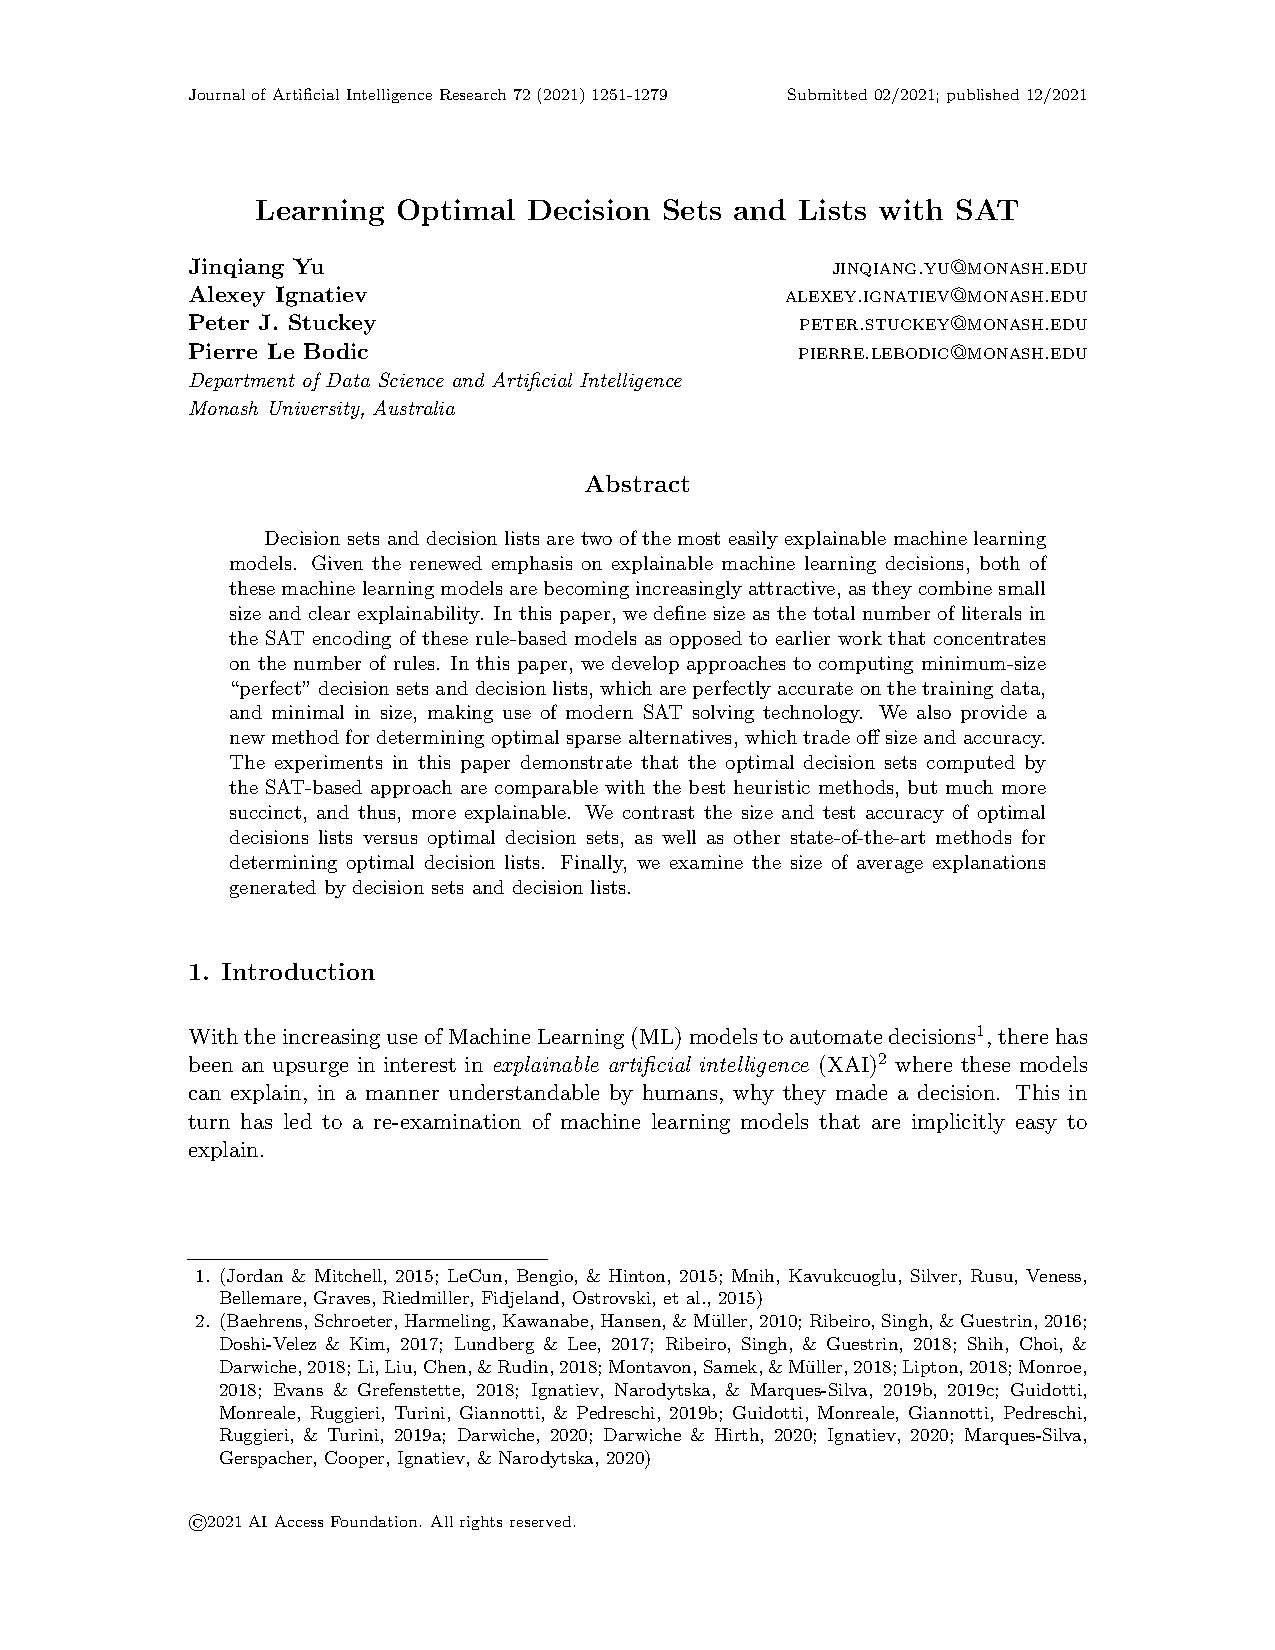
\includepdf[pages=-, offset=75 -75]{papers/jair21.pdf}
  
\chapter{From formal boosted tree explanations to
interpretable rule sets} \label{chap:cp23}

This chapter is based on:
\begin{itemize}
	\item Jinqiang Yu, Alexey Ignatiev, and Peter J. Stuckey. From formal boosted tree explanations to
interpretable rule sets. \emph{In 29th International Conference on Principles and Practice of
	Constraint Programming,} vol. 280, pp.38:1-38:21, 2023.
\end{itemize}

Explaining decision sets is notably straightforward: the rule that ``fires'' a given instance
serves as the explanation for that instance.
%
This led to increased interest in decision sets that are both easy to understand
to accurate.
%
The method presented in \autoref{chap:jair21} produces decision sets of minimum size that achieve
perfect accuracy on the training data and demonstrates that decision sets that fully align with the
training data exhibit superior accuracy compared to others.
%
A more scalable method~\cite{ilsms-aaai21} to generate perfectly accurate decision sets was the
introduced.
%
However, neither of these methods can offer any decision information if a dataset is not entirely solved.
%
Inspired by these studies and their limitations, this chapter focuses on establish a connection between 
formal post-hoc explainability and decision sets.
%
Specifically, this chapter aims to develop an innovative anytime method to generate decision sets that are 
both accurate and interpretable. 
%
This is achieved by distilling a gradient boosted tree model into a decision set on demand with 
the use of abductive explanations~(AXp's).
%
In addition, the chapter introduces several post-hoc model reduction techniques aimed at
improving the interpretability of the result decision sets with the use of MaxSAT and 
integer linear programming~(ILP).
%
Empirical results conducted on various datasets show that our method 
generates decision sets outperforming those produced by state-of-the-art approaches in terms of
accuracy, while remaining comparable regarding explanation size.


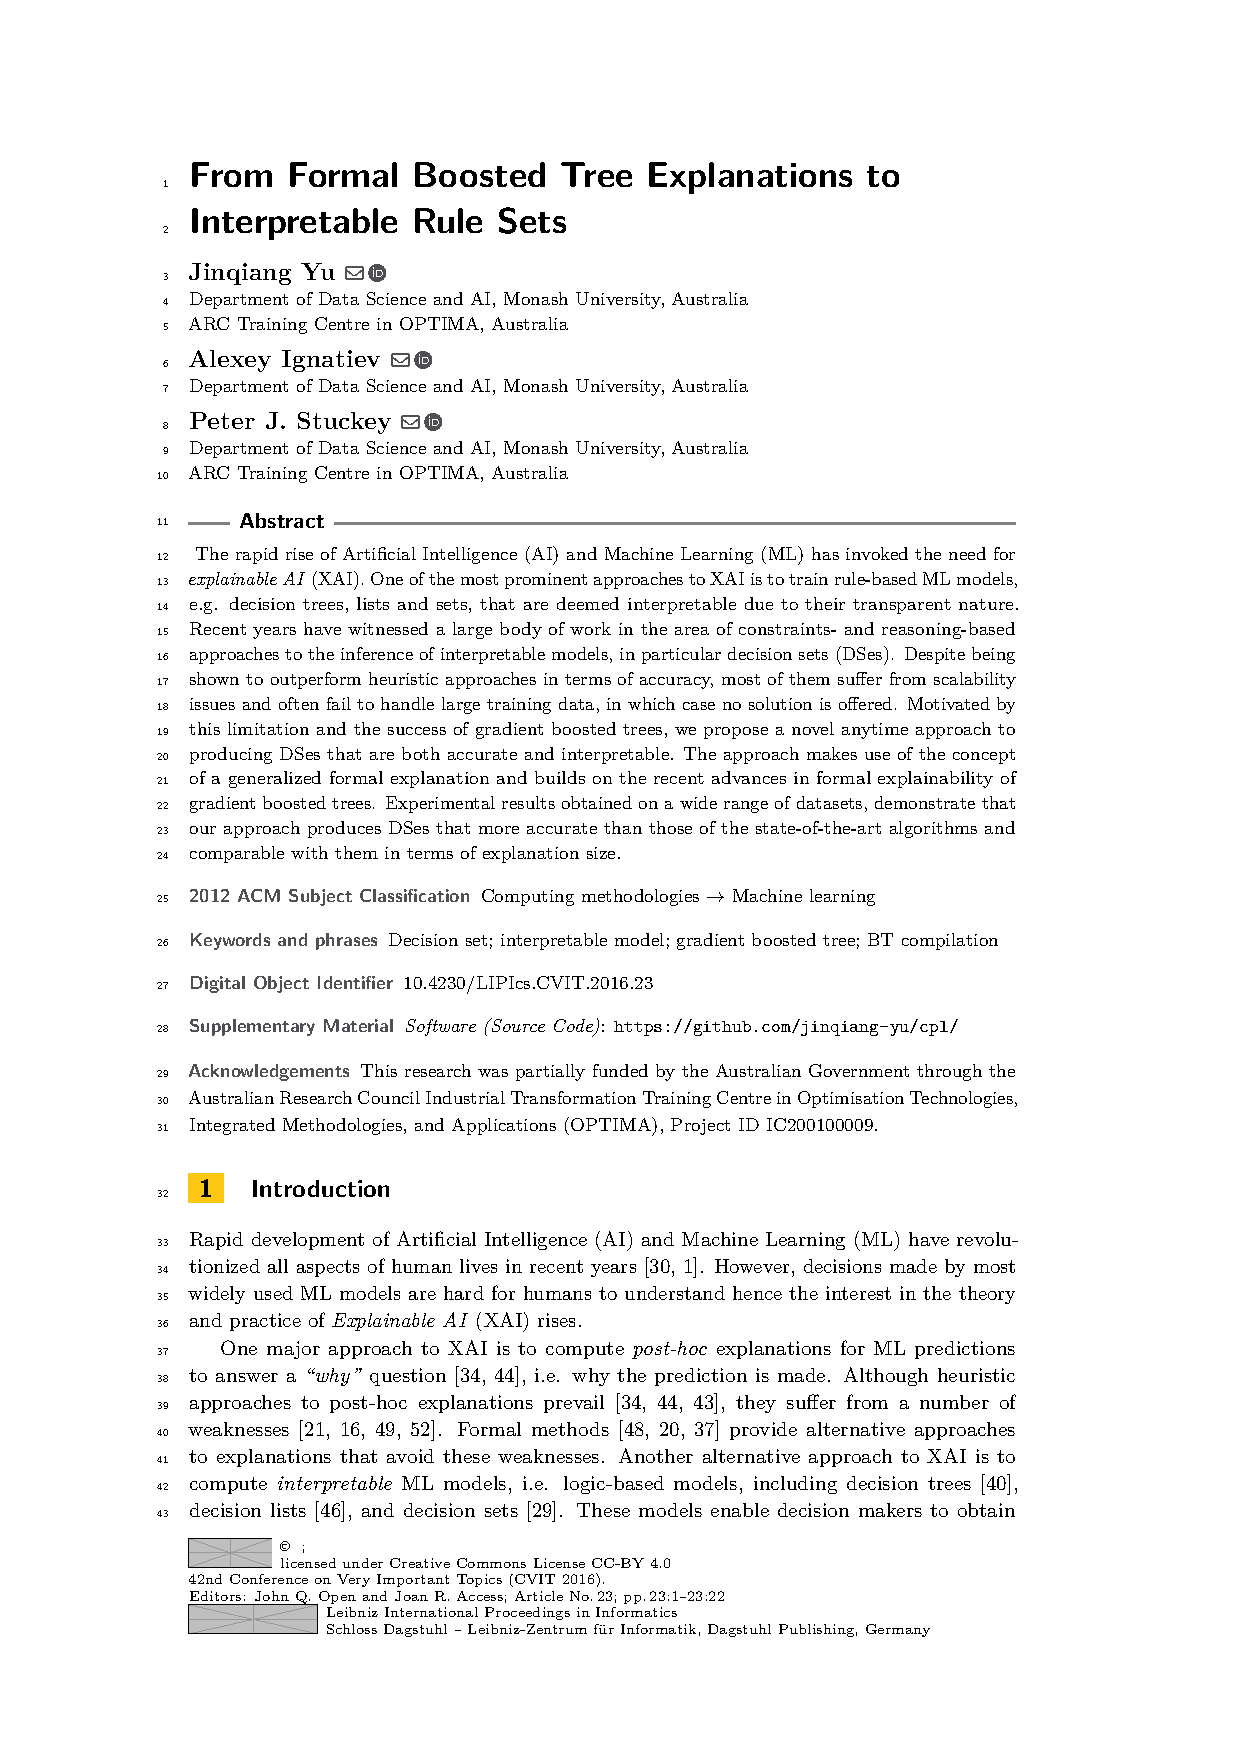
\includepdf[pages=-, offset=75 -75]{papers/cp23.pdf}
  
%\chapter{Eliminating The Impossible, Whatever Remains Must Be True}\label{chap:aaai23}
\chapter{Extracting and Applying Background Knowledge in the Context of Formal Explanations}
\label{chap:aaai23}

This chapter is based on:
\begin{itemize}
	\item Jinqiang Yu, Alexey Ignatiev, Peter J. Stuckey, Nina Narodytska, and Joao Marques-Silva.
Eliminating the impossible, whatever remains must be true: On extracting and applying background
knowledge in the context of formal explanations. \emph{In Proceedings of the AAAI Conference on Artificial
Intelligence,} vol. 37, pp. 4123-4131, 2023.
\end{itemize}

While the formal explainability method provides provably correct and minimal explanations,
a few limitations have been identified.
%
For instance, to ensure provable correctness of explanations, formal methods must consider the entire feature space, 
assuming that features are uniformly distributed and independent~\cite{kutyniok-jair21}.
%
This requires a formal reasoner to examine all potential combinations of feature values, 
even those that are unlikely to occur in practical contexts.
%
While this ensures the correctness of abductive explanations~(AXp's), it may result in unnecessarily
long explanations.
%
Additionally, it raises concerns about the validity of contrastive explanations~(CXp's), 
as the counterexamples they depend on may be not meaningful.
%
Inspired by the limitation, this chapter is aimed at generating both AXp's and CXp's
using background knowledge and presents the following contributions.
%
First, this chapter introduces an efficient method to mine background 
knowledge represented by precise if-then rules for a given training
dataset.
%
This method builds on a recent technique to learn decision 
sets~\cite{ilsms-aaai21}.
%
Second, we presents a novel method to produce AXp's and CXp's subject to extracted background knowledge. 
%
Also, this chapter theoretically demonstrates that incorporating background knowledge 
enhances the quality of both AXp's and CXp's, and therefore helps establish trust in the underlying AI systems.
%
Finally, inspired by~\cite{ignatiev-ijcai20}, we argue that background knowledge 
facilitates a more precise assessment of the correctness of model-agnostic 
explainers by preventing the consideration of impossible combinations of feature values.


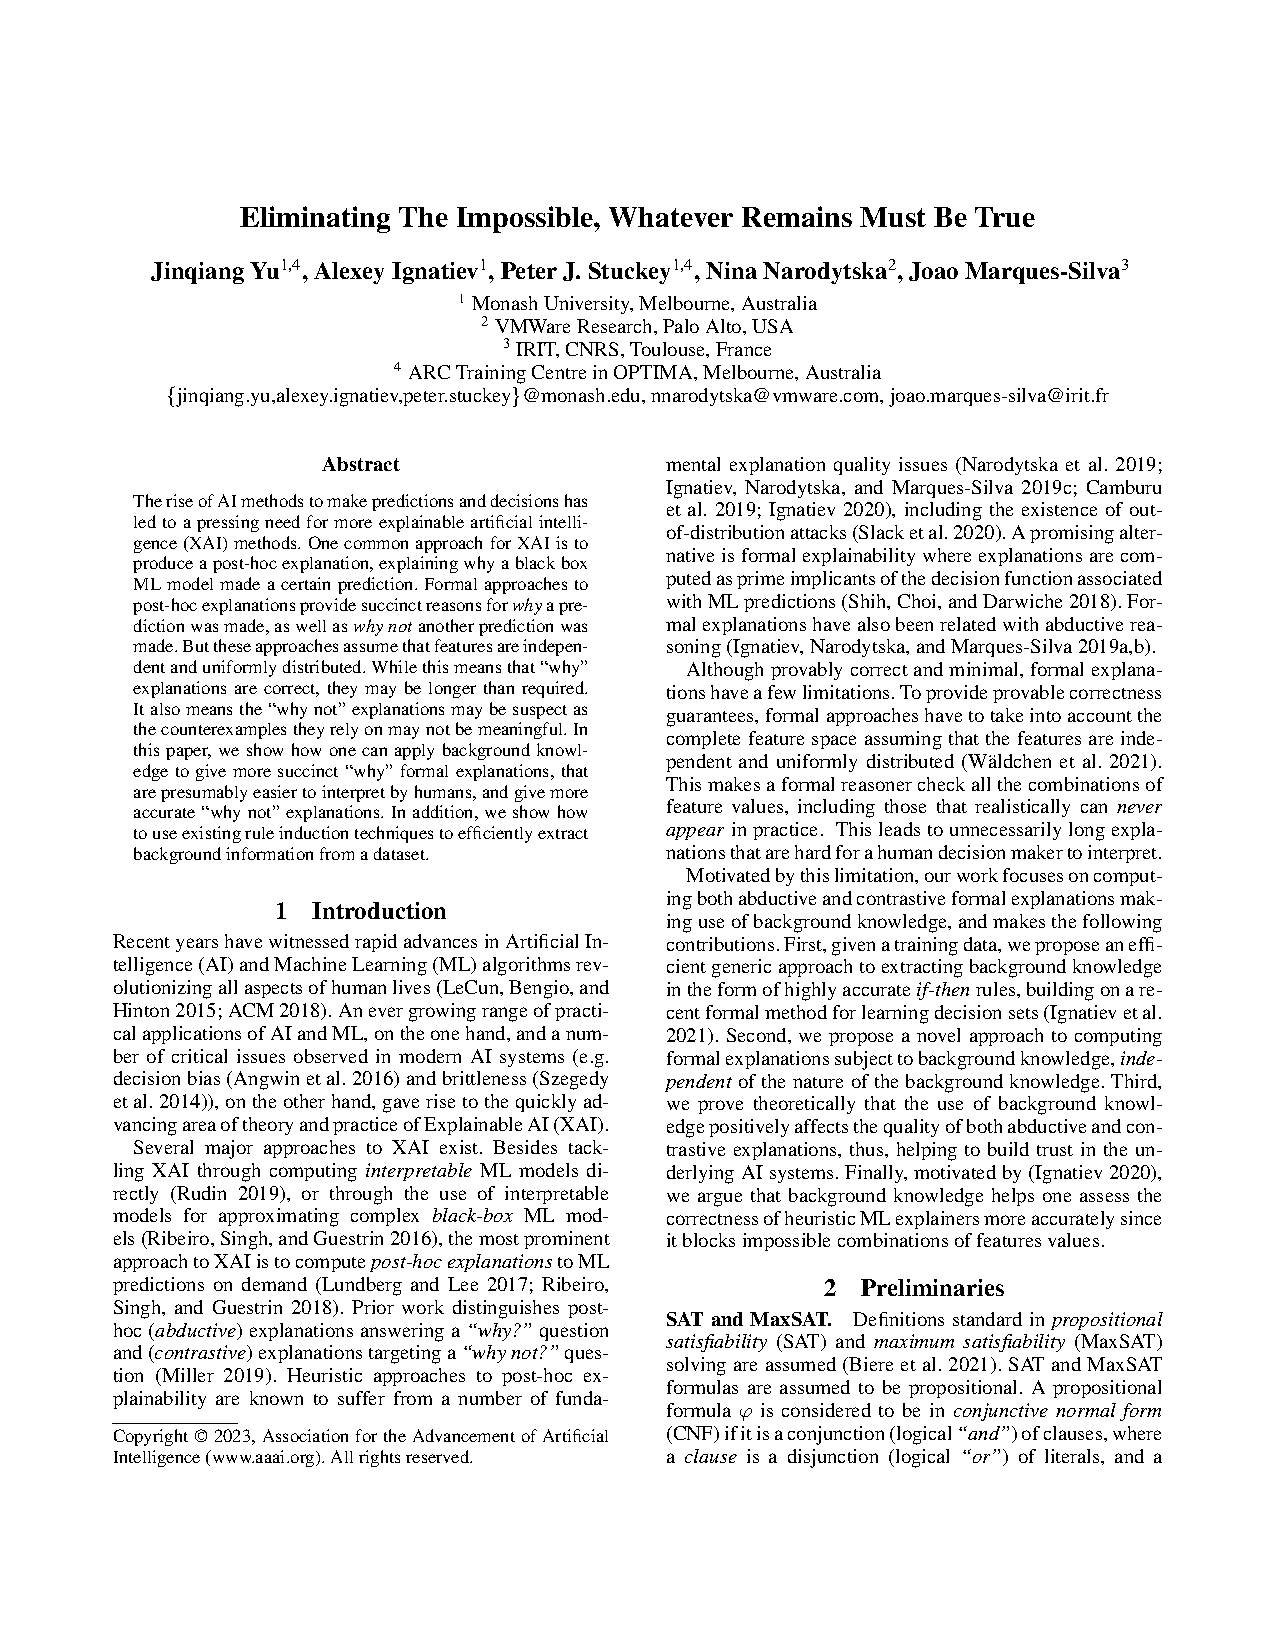
\includepdf[pages=-, offset=75 -75]{papers/aaai23.pdf}
  
\chapter{On Formal Feature Attribution and Its Approximation}\label{chap:ffa}


This chapter is based on:
\begin{itemize}
	\item Jinqiang Yu, Alexey Ignatiev, and Peter J. Stuckey. On Formal Feature Attribution and Its
Approximation. \emph{arXiv preprint arXiv:2307.03380,} 2023.
\end{itemize}

Serving as the alternative of model-agnostic XAI methods, 
formal XAI~(FXAI) approaches suffer from their own drawbacks,
such as scalability issues and the need to construct a logical representation
of ML models.
%
Also, formal explanations are often larger compared to their model-agnostic counterparts
as they do not take into account the reasoning about~(unknown) data distributions.
%
Lastly, and notably, FXAI approaches have not been applied to address feature attribution problems.
%
Motivated by the aforementioned limitations, this chapter introduces a 
novel formal method to generate feature attribution, 
leveraging the achievements of established FXAI techniques~\cite{msi-aaai22}.
%
Through exhaustive enumeration of all AXp's, we can define formal feature attribution~(FFA) as
the proportion of occurrences of a given feature within these AXp's.
%
Arguably, computing formal feature attribution is hard for the second level of the polynomial hierarchy.
%
While computing \emph{exact} FFA can be challening,
this chapter demonstrates that existing anytime formal explanation enumeration techniques can be
effectively used to approximate FFA.
%
Empirical results conduced on publicly accessible tabular and image datasets
show the practical effectiveness of the proposed method and its advantage
over SHAP and LIME, as well as in a real-world application of XAI in the field of 
software engineering~\cite{mcintosh2017fix,pornprasit2021pyexplainer}.


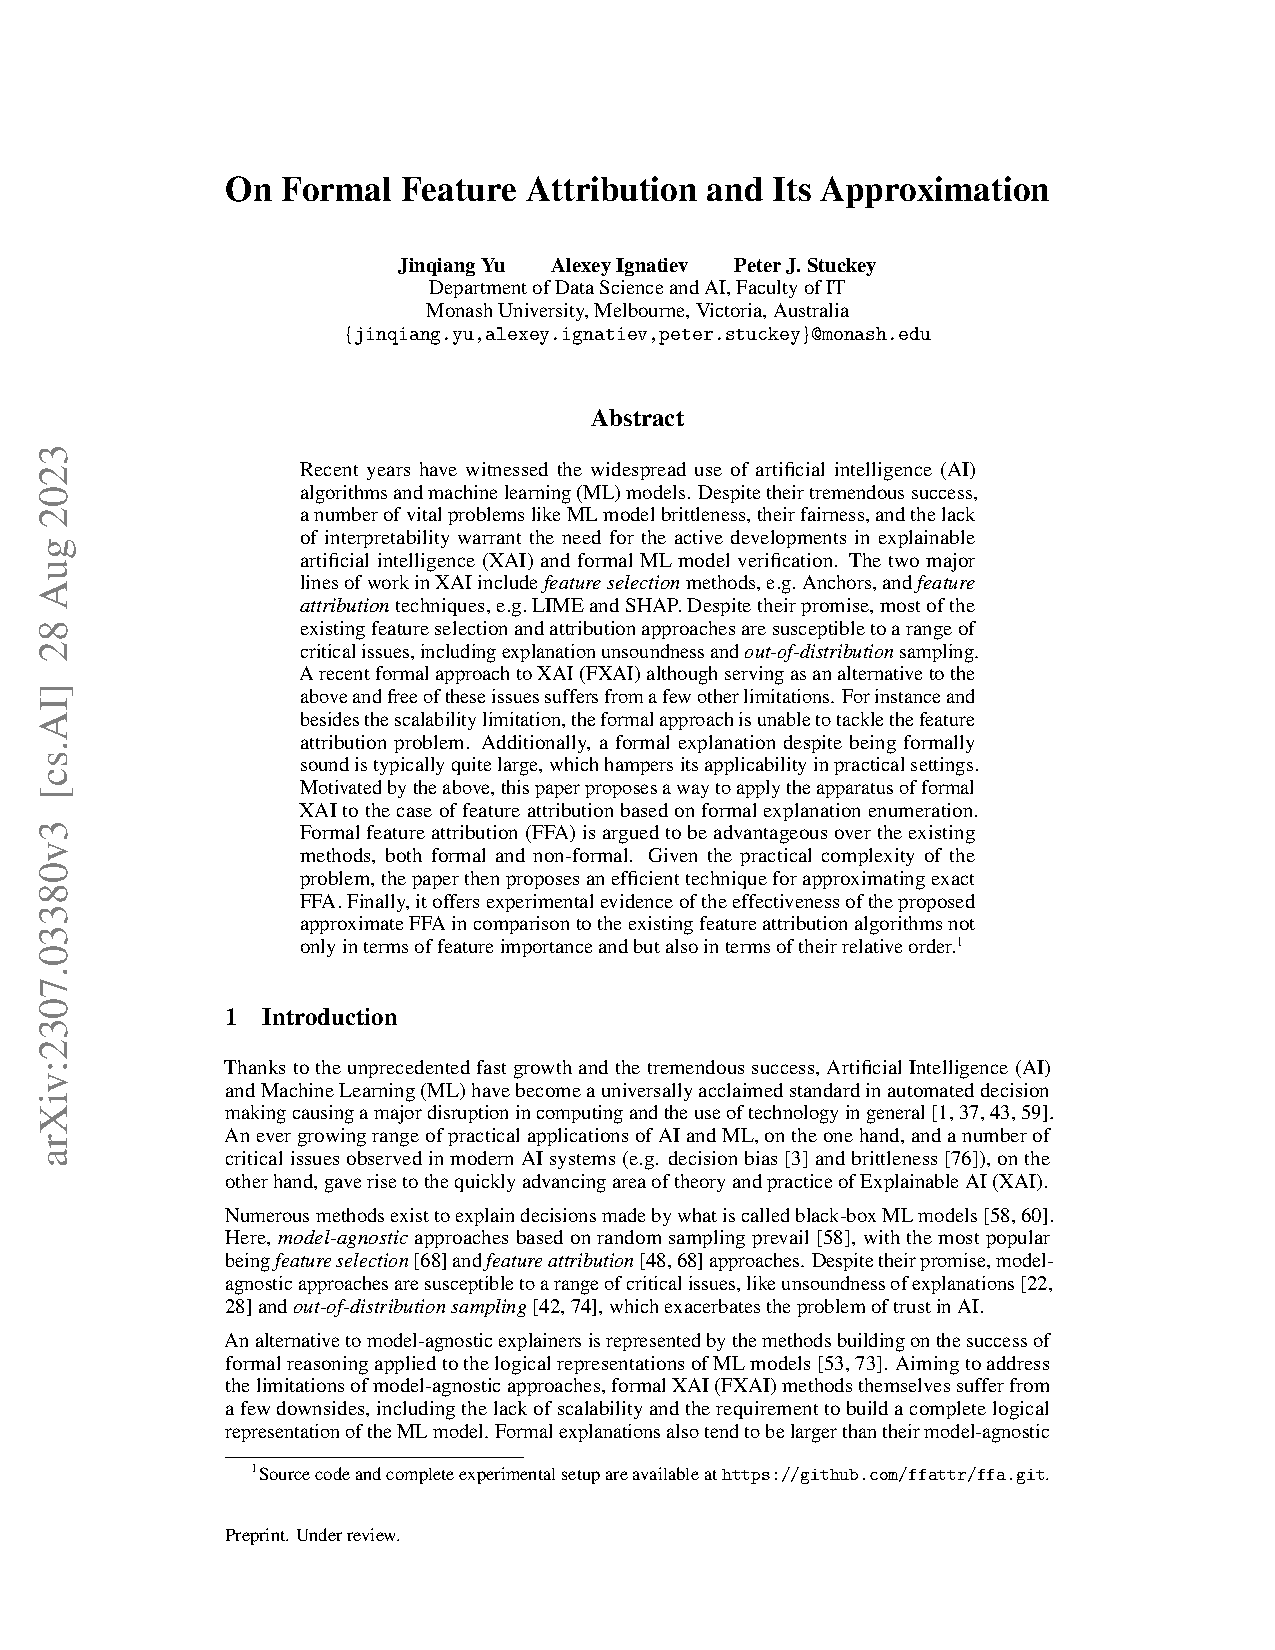
\includepdf[pages=-, offset=75 -75]{papers/ffa.pdf}
  
\chapter{Anytime Approximate Formal Feature Attribution}\label{chap:marco}


This chapter is based on:
\begin{itemize}
	\item Jinqiang Yu, Graham Farr, Alexey Ignatiev, and Peter J. Stuckey. Anytime Approximate Formal
Feature Attribution. \emph{arXiv preprint arXiv:2312.06973,} 2023.
\end{itemize}

\autoref{chap:ffa} provides a clear and crisp definition of FFA, but its computation presents
challenges,
since determining whether a feature has a non-zero attribution is as
least as hard as determining its relevance.
%
In \autoref{chap:ffa}, we demonstrate that FFA computation can be efficiently achieved 
by leveraging the hitting set duality between AXp's and CXp's.
%
While attempting to enumerate CXp's, a side effect of the algorithm is 
the discovery of AXp's. 
%
Indeed, the algorithm typically identifies numerous AXp's before encountering the first CXp.
%
In this case, the AXp's at the beginning are ensured to be diverse, as they must be broad in scope
to guarantee that the CXp is large enough to hit all relevant AXp's for exact FFA.
%
Therefore, collecting AXp's as side effects of CXp enumeration proves effective in the 
initial stages of the enumeration process.
%
However, as we collect an increasing number of AXp's as side effects, we eventually 
reach some point where significantly more CXp's are generated than AXp's.
%
Experimental results indicate that if we aim to enumerate all AXp's, it is preferable not to 
depend on the side effect behavior, but rather to directly enumerate AXp's.
%
This presents a dilemma: for fast and accurate approximations of FFA, we enumerate CXp's and
generate AXp's as a side effect, while to produce exact FFA, we compute all AXp's, and it is more 
advantageous to directly enumerate them.
%
In this chapter, we introduce an anytime method to produce approximate FFA,
where we initially enumerate CXp's and then switch to AXp enumeration dynamically 
when the rate of AXp discovery through CXp enumeration decrease.
%
Thus, we can quickly obtain accurate approximations while also accelerating the process of 
arriving at the complete set of AXp's compared to pure CXp enumeration.
%
The second contribution of this work involves exploring this alternative approach 
and demonstrating that even with a(n) (in)complete set of CXp's provided, 
determining FFA remains computationally challenging, as it is \#P-hard even when 
all CXp's are of size two.


%As direct CXp enumeration is feasible to do without the need to resort
%to the hitting set duality~\cite{msi-aaai22}, one may want to estimate
%FFA by first enumerating CXp's.
%

%The second contribution of this paper is to investigate this
%alternative approach and to show that even if a(n) (in)complete set of
%CXp's is given, determining FFA is computationally expensive being
%\#P-hard even if all CXp's are of size two.

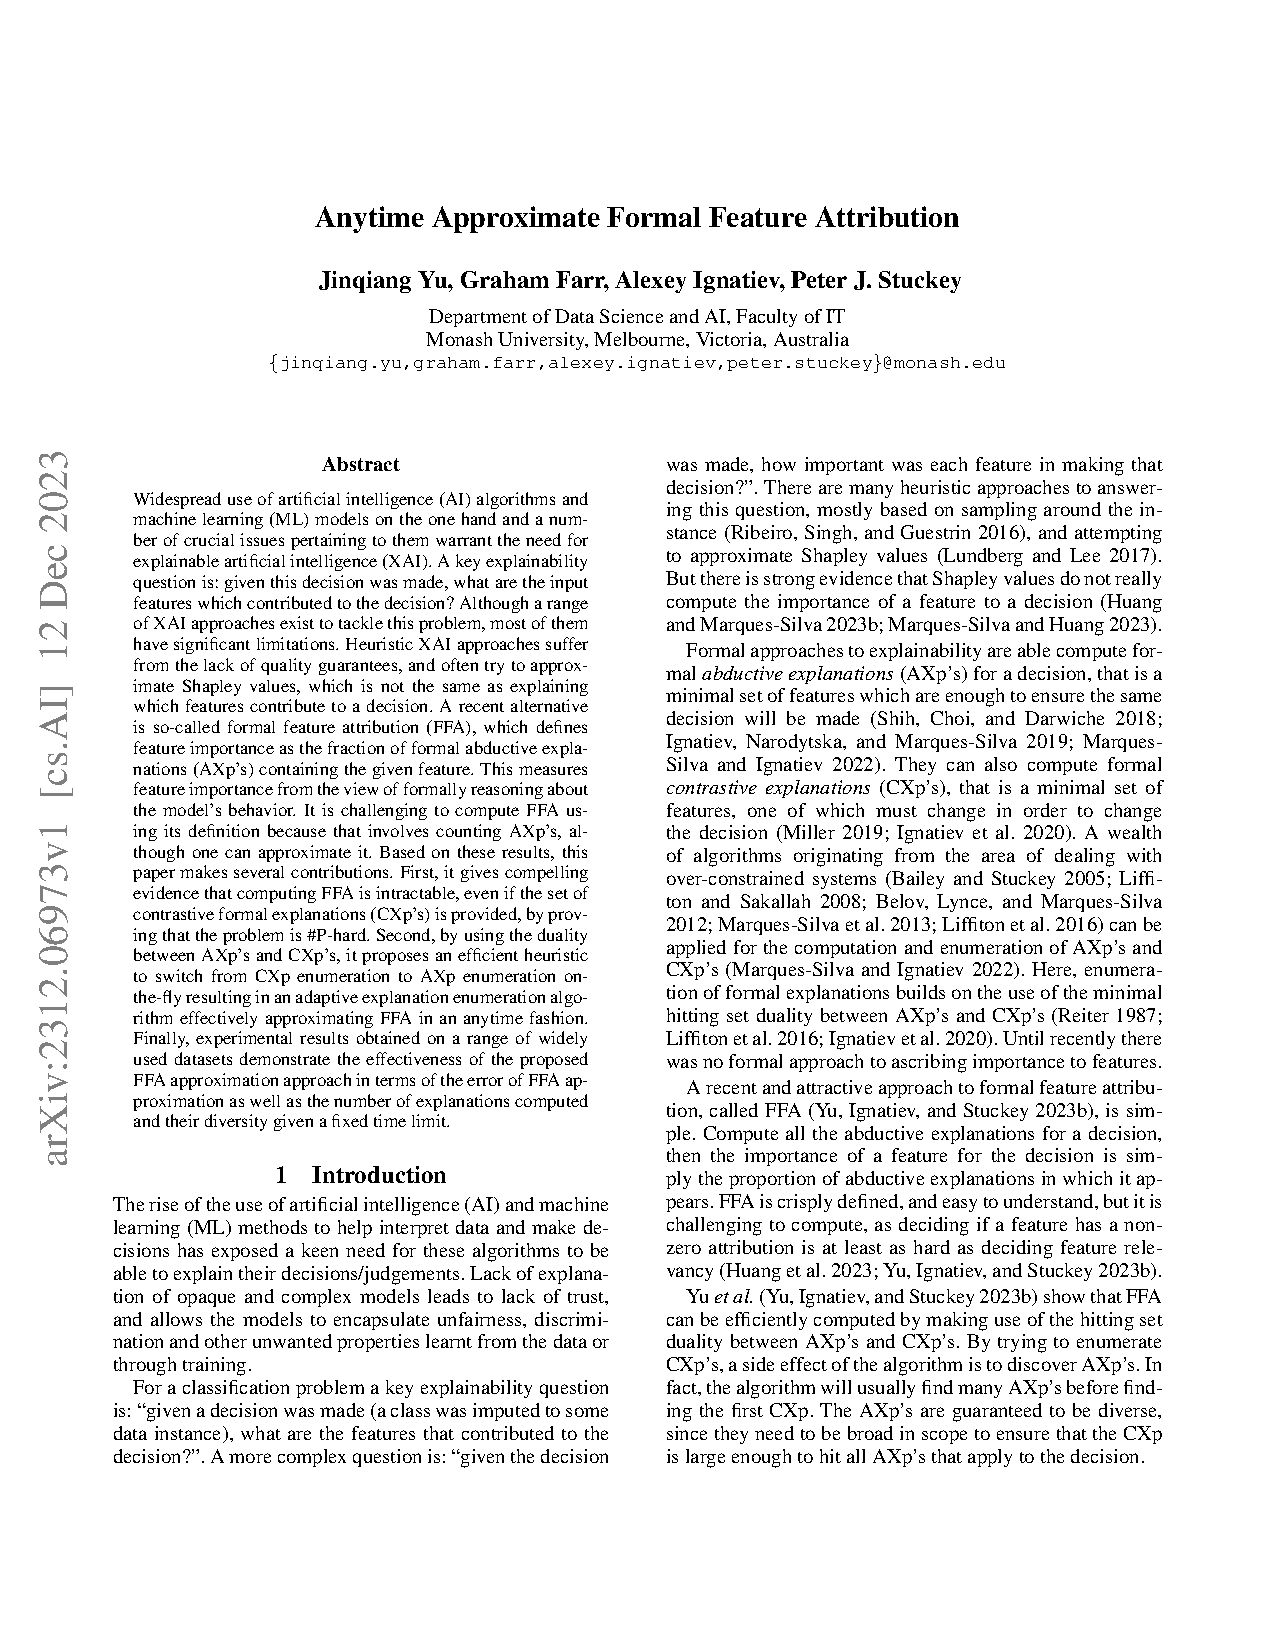
\includepdf[pages=-, offset=75 -75]{papers/marco.pdf}
  
\chapter{A Formal Explainer for Just-In-Time Defect Predictions}\label{chap:jit}

This chapter is based on:
\begin{itemize}
	\item Jinqiang Yu, Michael Fu, Alexey Ignatiev, Chakkrit Tantithamthavorn, and Peter J. Stuckey. A
Formal Explainer for Just-In-Time Defect Predictions. \emph{ACM Transactions on Software Engineering
	and Methodology,} 2024. (\textbf{Accepted.})
\end{itemize}

Software companies often rapidly release software products at a rapid pace in short-term development
cycles.
%
The rapid pace of software release presents significant challenges
because of the exponential increase of highly complex source code, particularly for 
under-resourced software quality assurance~(SQA) teams.
%
Due to the time-consuming and costly nature of various SQA activities, 
e.g., code review, developers are unable to thoroughly guarantee the highest quality for 
all newly developed code commits or pull requests given limited time and resources.
%
Just-in-Time (JIT) defect prediction~\cite{kim2007predicting,Kamei2013,pornprasit2021jitline,lin2021impact} is 
proposed to predict whether a commit will introduce software defects in the future. 
%
This allows teams to allocate their finite SQA resources to the most critical 
commits or pull requests. 
%
However, JIT defect prediction largely remains a black-box approach, 
offering predictions that lack explainability and actionable insights for practitioners.
%
Previous research has applied a range of model-agnostic techniques to explain the predictions made
by JIT models.
%
Unfortunately, explanations produced by these methods are still not formally sound, robust, and
actionable.
%
Motivated by the limitation of model-agnostic approaches, this chapter introduces FoX, 
a Formal eXplainer for JIT defect prediction.
%
With the use of formal reasoning about the functionality of JIT defect prediction models,
FoX can offer explanations that are not only provably correct but also guaranteed to be 
minimal.
%
Experimental results demonstrate that FoX can effectively produce explanations that are provably correct, correct,
and actionable. 
%
In contrast, explanations generated by model-agnostic methods do not hold this
%
The survey conducted among 54 software practitioners offers valuable insights 
into the usefulness and trustworthiness of FoX.
%
74\% of respondents found it to be trustworthy,
and 86\% agreed with the usefulness of FoX.
%
Hence, this chapter serves as a significant advancement towards providing trustable explanations for
JIT models, enabling domain experts and practitioners to gain a clearer understanding of
why a commit is predicted as defective and how to mitigate the risk.

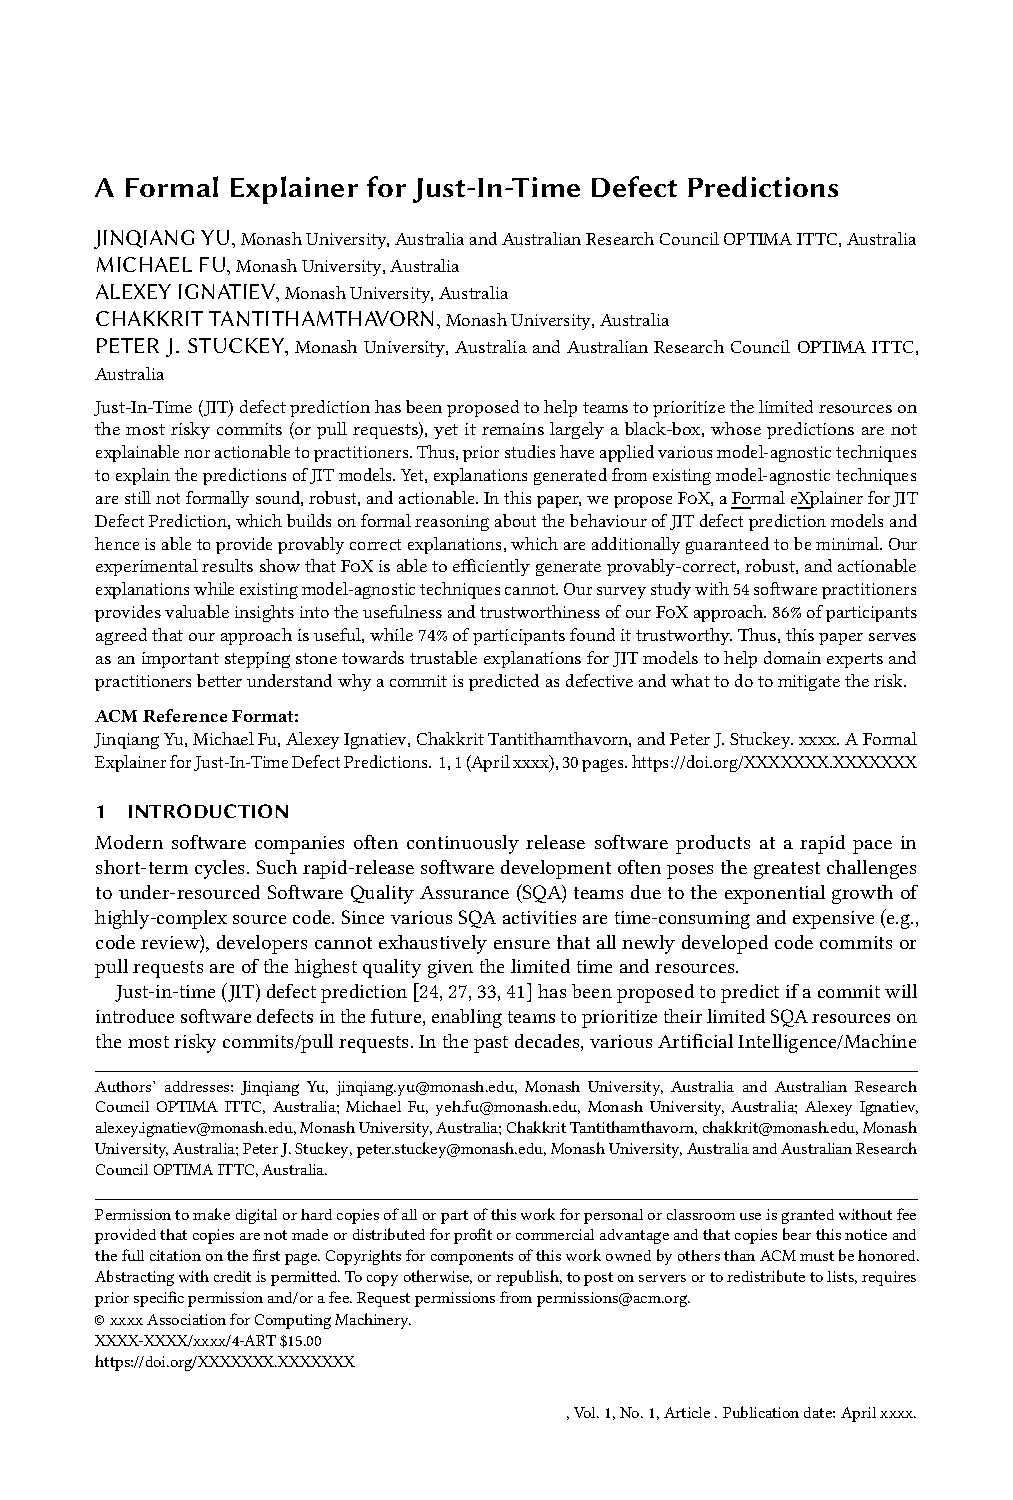
\includepdf[pages=-, offset=75 -75]{papers/jit.pdf}
  
\chapter{Conclusions and Future Work}\label{chap:conc}

\section*{Conclusions}

% growing XAI and its application in various domains
% model-agnostic and FXAI
%

While machine learning~(ML) and Artificial Intelligence~(AI) \newmm{advances} have been 
widely applied across diverse domains like finance, 
the lack of transparency in these systems triggers significant concerns, 
e.g. fairness, bias, safety and robustness.
%
As a result, there is a growing interest of eXplainable AI~(XAI) aimed to establish trust in \newmm{ML/AI} 
systems, by explaining or illustrating the behavior of ML models in 
human-understandable ways.
%
Among various approaches to XAI, model-agnostic approaches
stand out as the prevailing ones although they encounter challenges regarding 
the quality of generated explanations. 
%
As an alternative, formal XAI~(FXAI) methods offer logic-based or formal explanations, 
aimed to provide provable and robust explanations for ML predictions.
%
This thesis concentrates on XAI challenges, especially formal explainability,
\newmm{trying enhancing} the interpretability of ML models
and addressing gaps in formal explainability.
%
The primary contributions of this thesis are outlined as follows:

% contributions again
\begin{itemize}
	\item \autoref{chap:jair21} introduces methods to generate decision sets and decision lists 
		that are optimal either in terms of the number of required literals or 
		the trade-off between model size and accuracy.
		%
		In this study, we define size as the total number literals used in these rule-based ML models,
		in contrast with previous research that primarily focuses on the number of rules in
		the model, which cannot adequately capture the explainability of such models.
		%
		The empirical results illustrate that the decision sets and lists computed by the
		proposed approaches are able to achieve decent trade-off between interpretability (represented by model size) and accuracy.

	\item In \autoref{chap:cp23}, we present an innovative anytime approach to producing decision sets
		through the on-demand extraction of generalized abductive explanations for boosted
		trees.
		%
		The proposed method can be used to compile a gradient boosted tree
		with respect to either the complete feature space, or a set of
		target training instances.
		%
		Augmented by post-hoc model size reduction approaches, 
		this method is demonstrated to generate decision sets that outperform those
		computed by state-of-the-art algorithms in terms of accuracy and remain 
		comparable with them regarding explanation size.
		%
		Note that the presented method can be categorized as a knowledge distillation technique and theoretically, 
		it can extend to any other ML models.

	\item In \autoref{chap:aaai23}, we propose a technique to apply background knowledge to enhance 
		the quality of explanations. 
		%
		There are substantial advantages of incorporating background knowledge in generating
		formal explanations for ML models.
		%
		In the context of abductive explanations~(AXp's), 
		integrating background knowledge significantly reduces the length of explanations, 
		making them more explainable, and improve the efficiency of explanation generation.
		%
		In the case of contrastive explanations (CXps), although applying background knowledge may 
		increase the explanation size and potentially require more time for explanation generation, 
		the resulting explanations are significantly more precise because they do not 
		depend on the (often unsupportable) assumption that all tuples in the feature space 
		are feasible.
		%
		Moreover, as demonstrated in \autoref{chap:aaai23}, background knowledge can be 
		integrated into the context of heuristic explanations, particularly when an accurate
		analysis of is need.

	\item \autoref{chap:ffa}  introduces the first method for formal feature attribution~(FFA),
		using the proportion of abductive explanations where a feature appears to
		indicate its significance.
		%
		Experimental results demonstrate that we can compute exact FFA for numerous classification tasks, 
		and in cases where exact computation is infeasible, we can compute effective approximations.
		%
		Additionally, we found existing model-agnostic method to generate to feature attribution 
		disagree with FFA.
		%
		In some cases, they are considerably different from FFA, such as assigning no weight to 
		a feature that is present in (a significant number of) explanations,
		or assigning a (large) non-zero weight to a feature that holds no relevance for the prediction.
		%
		Overall, \autoref{chap:ffa} argues that if we acknowledge FFA as a valid measure 
		of feature attribution, it is important to explore approaches that generate good 
		approximate FFA more efficiently.

	\item In \autoref{chap:marco}, motivated by the difficulty of exact computation for 
		many classifiers and datasets, we introduce an anytime method for FFA
		approximation.
		%
		As illustrated in this chapter, computing FFA remains challenging even 
		when the set of CXp's is available. 
		%
		Therefore, there is a demand for anytime method to generate FFA.
		%
		Surprisingly, starting with CXp enumeration to produce AXps results in 
		rapidly achieving good approximations of FFA.
		%
		However, in the longer turn this method proves to be less effective 
		compared to simply enumerating AXps.
		%
		This work demonstrates the integration of these approaches by strategically 
		switching the enumeration phase, ensuring that information computed in the 
		underlying MARCO enumeration algorithm is preserved.
		%
		This presents a highly practical method to generate \newmm{or approximate} FFA.

	\item \autoref{chap:jit} introduces the first formal explainer for just-in-time~(JIT) 
		defect prediction. 
		%
		This novel explainer leverages formal reasoning by exploiting propositional logic
		to efficiently produce explanations that are provably correct, robust, 
		and subset-minimal, addressing ``why'' questions, such as why a commit is 
		predicted as defective.
		%
		The proposed formal explainer is also capable of producing contrastive ``how'' 
		explanations that are provably correct, robust, and subset-minimal, 
		offering more actionable insights compared to abductive explanations.
		%
		This marks a significant step towards actionable software analytics.
		%
		Therefore, these generated explanations are able to assist researchers 
		in designing actionable defect prediction methods and help practitioner direct their
		attention towards the most crucial aspects related to software defects. 
		%
		This, in turn, enhances the operational decision-making of software quality assurance~(SQA) teams.
\end{itemize}

\section*{Feature work}
While this thesis presents numerous \newmm{advances} in the field of XAI, 
there are still several directions that need to be addressed in future research.
%
Some future directions are outlined as follows.

\textbf{Applying Formal Explainability}.
%
Although ML and AI are widely used in diverse fields, such as healthcare, law, finance, and transportation, 
the opacity of \newmm{ML/AI} systems can hinder users from gaining clear insights into 
the outputs produced by these systems.
%
Consequently, these systems fail to establish trust between humans and the
predictions generated by ML models.
%
Inspired by the limitation, in \autoref{chap:jit} we \newm{apply} formal explainability for
just-in-time~(JIT) defect prediction, aiming to establish trust for the predictions.
%
To broaden the applicability of ML and AI applications, one future research direction 
will focus on applying formal explainability across various fields.
%
This will help users trust the predictions generated by ML models, facilitating the wider 
adoption of ML and AI in diverse domains.

\textbf{Improving Scalability of Formal Explainability}.
%
With the increasing need to deploy large and complex \newmm{ML/AI} systems across diverse domains, 
the scalability of XAI approaches has emerged as a notable concern.
%
Unfortunately, formal explainability encounters scalability challenges, 
particularly with certain complex classifier families, such as neural networks.
%
These models are computationally expensive or hard to reason formally
to produce formal explanations due to their complex structure.
%
To address this scalability limitation, recent research~\cite{bk-tacas23} 
suggests a novel method to approximate formal explanations, with the use of 
technologies aimed at evaluating the robustness of neural networks.
%
Additionally, recent research~\cite{bk-tacas23} introduces innovative algorithms for computing
formal explanations, achieved by finding a direct relationship between 
the practical complexity of robustness and formal explainability.
%
Inspired by the scalability issue and these studies, one feature research direction
will focus on developing methods to efficiently
generate formal explanations for complex ML models.
 % Conclusions  



%% ----------------------------------------------------------------
% Now begin the Appendices, including them as separate files

%\addtocontents{toc}{\vspace{2em}} % Add a gap in the Contents, for aesthetics
%
%\appendix % Cue to tell LaTeX that the following 'chapters' are Appendices
%
%\input{Appendices/AppendixA}	% Appendix Title

%\input{Appendices/AppendixB} % Appendix Title

%\input{Appendices/AppendixC} % Appendix Title

\addtocontents{toc}{\vspace{2em}}  % Add a gap in the Contents, for aesthetics
\backmatter

%% ----------------------------------------------------------------
\label{Bibliography}
\lhead{\emph{Bibliography}}  % Change the left side page header to "Bibliography"
%\bibliographystyle{unsrtnat}  % Use the "unsrtnat" BibTeX style for formatting the Bibliography
\bibliographystyle{plainnat} 
\bibliography{bib}  % The references (bibliography) information are stored in the file named "Bibliography.bib"

\end{document}  % The End
%% ----------------------------------------------------------------
